%!TEX root = Thesis.tex

\chapter{Coordination Complexes with Rhodium and Iridium}
\chaptermark{Rhodium and Iridium}
\label{ch:rhodium}

Rhodium is a very rare element forming only 0.001 ppm of the earth's crust.\cite{Enghag2004Rhabundance}  The majority of the extracted rhodium (81\%) is used in catalytic converters to reduce harmful nitrogen oxides to nitrogen and oxygen.  Another important use of rhodium is in thermocouples where a rhodium-platinum alloyed wire is used, together with a pure platinum wire for use in high-temperature furnaces.\cite{Enghag2004Rh}  Rhodium coordination complexes form active catalysts, most commonly for hydroformylation and hydrogenation.  Wilkinson's catalyst, \ce{[RhCl(PPh3)3]}, is one of the most widely known rhodium catalysts, used mainly for the hydrogenation of alkenes but also for hydroboration of alkenes and selective hydrogenation of $\alpha$-$\beta$-unsaturated carbonyl compounds.  

The 2001 Nobel Prize in Chemistry was awarded to Knowles,\cite{Knowles2002} Noyori\cite{Noyori2002} and Sharpless\cite{Sharpless2002} for their work in asymmetric catalysis, including several examples of rhodium catalysts.  A derivative of Wilkinson's catalyst where triphenylphosphine was replaced by the chiral phosphine (-)-\ce{PMePh^iPr} was reported by Knowles and Sabacky in 1968\cite{Knowles1968}.  This chiral version of Wilkinson's catalyst was the first asymmetric hydrogenation catalyst yielding an enantiomeric excess of 15\% when hydrogenating $\alpha$-$\beta$-unsaturated carbonyls (Scheme \ref{Knowlesscheme}).  This was improved upon by the development of the CAMP ligand (Figure \ref{chiralrhodiumligands}) which gives an enantiomeric excess of 80\% in the hydrogenation of dehydroamino acids, a key step in the commercial production of \iupac{\L-DOPA}  a drug used in the treatment of Parkinson's disease.\cite{Noyori2007}  Rhodium complexes containing chiral diphosphines also form active catalysts, for example a \iupac{[\cip{S}-BINAP}-Rh(COD)] (Figure \ref{chiralrhodiumligands}) catalyst is active for the asymmetric isomerisation of allylic amines a key step in the industrial synthesis of ($-$)-menthol generating over 1000 tons per year.\cite{Noyori2002}

\begin{scheme}[h]
\begin{center}
\vspace{0.5cm}
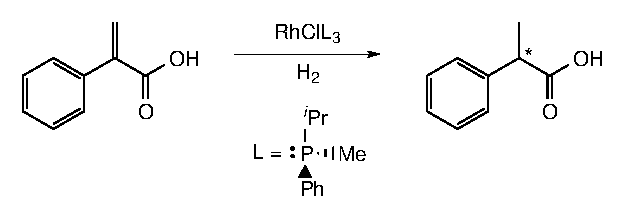
\includegraphics{../Schemes/Knowlesscheme.eps}
\caption[Asymmetric catalytic hydrogenation developed by Knowles]{Asymmetric catalytic hydrogenation developed by Knowles\cite{Knowles2002}}
\vspace{0.2cm} 
\label{Knowlesscheme}
\end{center}
\end{scheme}
\vspace{0.2cm}

\begin{figure}[h]
\begin{center}
\vspace{0.5cm}
	\begin{subfigure}{0.2\textwidth}
		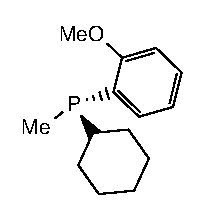
\includegraphics{../Structures/CAMP.eps}
	\end{subfigure}
	~~~~~~~~~~~~~~~~~~
	\begin{subfigure}{0.2\textwidth}
		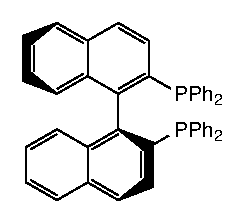
\includegraphics{../Structures/BINAP.eps}
	\end{subfigure}
\caption[Chiral phosphine ligands used in asymmetric catalysis]{Chiral phosphine ligands used in asymmetric catalysis.  Left: CAMP, Right: \iupac{\cip{S}-BINAP}}
\vspace{0.2cm}
\label{chiralrhodiumligands}
\end{center}
\end{figure}
\vspace{0.2cm}

%The xantphos class of ligands have long been studied for their role as ancillary ligands in  rhodium catalysed hydroformylation.  

The xantphos class of ligands were first studied for their potential use as ancillary ligands in rhodium catalysed hydroformylation\cite{Kranenburg1995}.  It was found that increasing the bite-angle from 108.7\degrees for sixantphos to 109.4 \degrees for thixantphos and 111.7 \degrees for xantphos resulted in an increase in the selectivity for the linear aldehyde (linear/branched = 35.0, 47.6 and 57.1 respectively).  A more recent paper with \iPrxantphos{} found a dramatic difference between the reactivity of the diphosphine towards rhodium and iridium.  Xantphos ligands have the ability to coordinate to a metal centre in a number of different modes.  The most common is the diphosphine \dento{2}-\emph{PP\textprime} mode.  Tridentate \POP{} complexes of the xantphos ligands are also relatively common especially in octahedral complexes.  In this case, the xantphos ligand most typically coordinates to the metal in a meridional mode, although facial complexes have also been reported.\cite{Dallanegra2012, Pawley2012}  Given the importance of the xantphos class of ligands to rhodium catalysis we chose to investigate the coordination chemistry of the \tBuxantphos{} ligands with rhodium.  

\section{Synthesis of [Rh(\tBuxantphosk)Cl] complexes}
\label{section:rhodiumchloride}

Rhodium alkene dimers are commonly used starting materials for the formation of rhodium phosphine complexes.  These dimers can react in a number of different ways depending on the phosphine (Figure \ref{RhCOEClcomplexes}).  When two equivalents of a monophosphine react with \ce{[Rh(COE)2Cl]2} the phosphine displaces one cyclooctene molecule from each rhodium forming a symmetric dimer.\cite{Canepa2003}  These complexes are typically unstable.  Further addition of phosphine displaces the remaining two cyclooctene molecules while retaining the chloride bridged rhodium core.\cite{Bleeke1986}  Analogous complexes form when the reaction is carried out with diphosphines.\cite{Fryzuk1989}  In some cases bidentate ligands can cleave the dimer resulting in a \ce{[Rh(LL)(COE)Cl]} complex.\cite{Hashimoto2010}  Tridentate ligands are able to cleave the dimer and result in the mononuclear complexes \ce{[Rh(LLL)Cl]}\cite{Khan1988, Hermann2002}.  In the case of negatively charged tridentate ligands the complex forms a trigonal bipyramidal hydride chloride structure (where the hydride forms from the central ligating atom).\cite{Boom1998, Winter2003, Salem2008}  Alternatively the ligand can be reacted first with a strong base or a silver salt can be added to remove the chloride and break the dimer.  In this case the remaining coordination site is occupied either by the anion from the silver salt, or by a cyclooctene molecule if a non-coordinating counterion is used.\cite{Fryzuk1986, Hanson2008}

\begin{figure}[h!]
\begin{center}
\vspace{0.5cm}
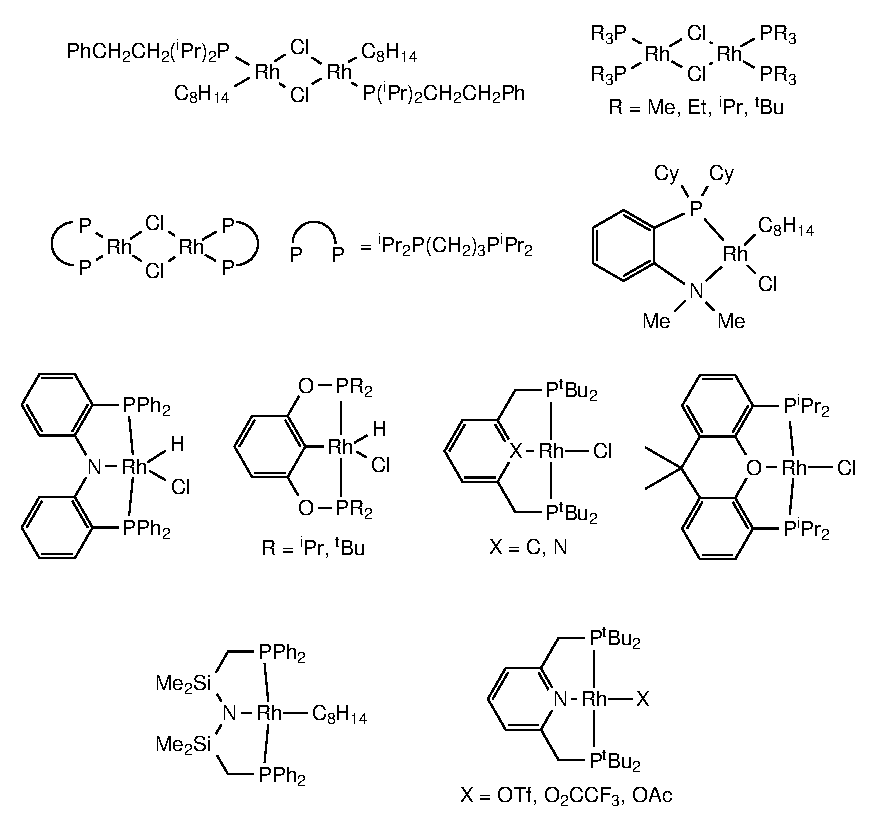
\includegraphics{../Figures/RhCOEClcomplexes.eps}
\caption[Complexes formed by reaction of \ce{[Rh(COE)2Cl]2} and phosphine ligands]{Complexes formed by reaction of \ce{[Rh(COE)2Cl]2} and phosphine ligands.  First row: monophosphines in 2:1 and 4:1 ligand:\ce{[Rh(COE)2Cl]2}, second row: bidentate ligands, third row: tridentate ligands in the absence of other reagents, fourth row: tridentate ligands using lithiated ligand (left) or a silver salt (right).}
\vspace{0.2cm}
\label{RhCOEClcomplexes}
\end{center}
\end{figure}
\vspace{0.2cm}

Reaction between \ce{[Rh(COE)2Cl]2} and the three \tBuxantphos{} ligands was carried out on an NMR scale in \ce{C6D6}.  No reaction occurred at room temperature overnight except in the case of \tBuxantphos{} which displays a small amount of conversion evident from the NMR spectra.  Upon heating to 60 \degC{} the reaction proceeds, going to completion after 24 hours.  For all three \tBuxantphos{} ligands the product is the expected [Rh(\tBuxantphosk)Cl] mononuclear complex (Scheme \ref{RhodiumI}).  This complex is directly analogous to the \iPrxantphos{} complex reported in 2013\cite{Esteruelas2013}.  As seen previously the \tBuxantphos{} ligands have a number of different coordination modes.  In this case a meridional \POP{} pincer coordination is observed.  It is likely the reaction proceeds by substitution of one cyclooctene ligand with one of the phosphorus atoms, followed by a second to form a chloride bridged dimer.  However, as the \tBuxantphos{} have such large bite-angles and the potential coordinating ether bridge this can readily split the dimer resulting in the desired product.  None of these intermediates were observable indicating low activation barriers once the first substitution had occurred.  

\begin{scheme}[htb]
\begin{center}
\vspace{0.5cm}
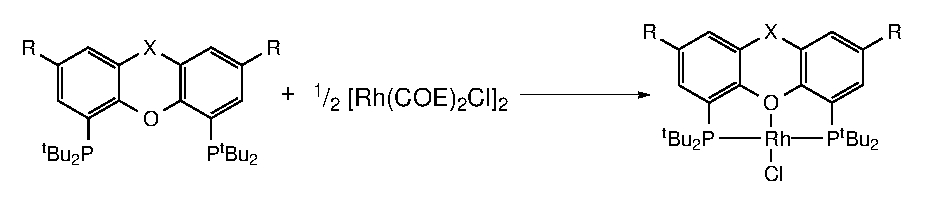
\includegraphics{../Schemes/RhodiumI.eps}
\caption[Reaction of \ce{[Rh(COE)2Cl]2} and \tBuxantphos{} ligands]{Reaction of \ce{[Rh(COE)2Cl]2} and \tBuxantphos{} ligands.  \tBuxantphos: R = H, X = \ce{CMe2}. \tButhixantphos: R = Me, X = S. \tBusixantphos: R = H, X = \ce{SiMe2}}
\vspace{0.2cm} 
\label{RhodiumI}
\end{center}
\end{scheme}
\vspace{0.2cm}

The NMR spectra for the three complexes is consistent with the proposed structures (spectra for [Rh(\tBuxantphos)Cl] shown in Figure \ref{RhClnmr}) .  In the phosphorus NMR spectra the complexes all display doublets due to rhodium coupling shifted downfield from the free ligand by 35.8-37.5 ppm to 44.2-47.7 ppm with coupling of 140-142.3 Hz (Table \ref{table:rhodiumchloride}).  This coupling is consistent with a rhodium(I) complex and is very close to the coupling for [Rh(\iPrxantphosk)Cl] complex (142.4)\cite{Esteruelas2013}  The \proton{} and \carbon{} NMR spectra support the proposed structure as the \tBu{} proton and carbons all appear as virtual triplets indicating strongly coupled phosphorus atoms which typically occurs in a \trans{} coordination geometry.  In the \carbon{} NMR the O-ipso carbon has shifted downfield relative to the free ligand and similar complexes where the oxygen is known to be non-coordinating [Ag\tBuxantphos)Cl].  This downfield shift is consistent with a coordinated oxygen.  As the oxygen donated electron density to the metal this will inductively decrease electron density on the O-ipso carbon resulting in decreased shielding and thus a downfield shift.  %The coupling on the O-ipso carbon decreases from the free ligand to a \dento{2}-\emph{PP\textprime} complex, but increases in the [Rh(\tBuxantphosk)Cl] complexes.  \fixme{why}

\begin{figure}[htbp]
\begin{center}
\vspace{0.5cm}
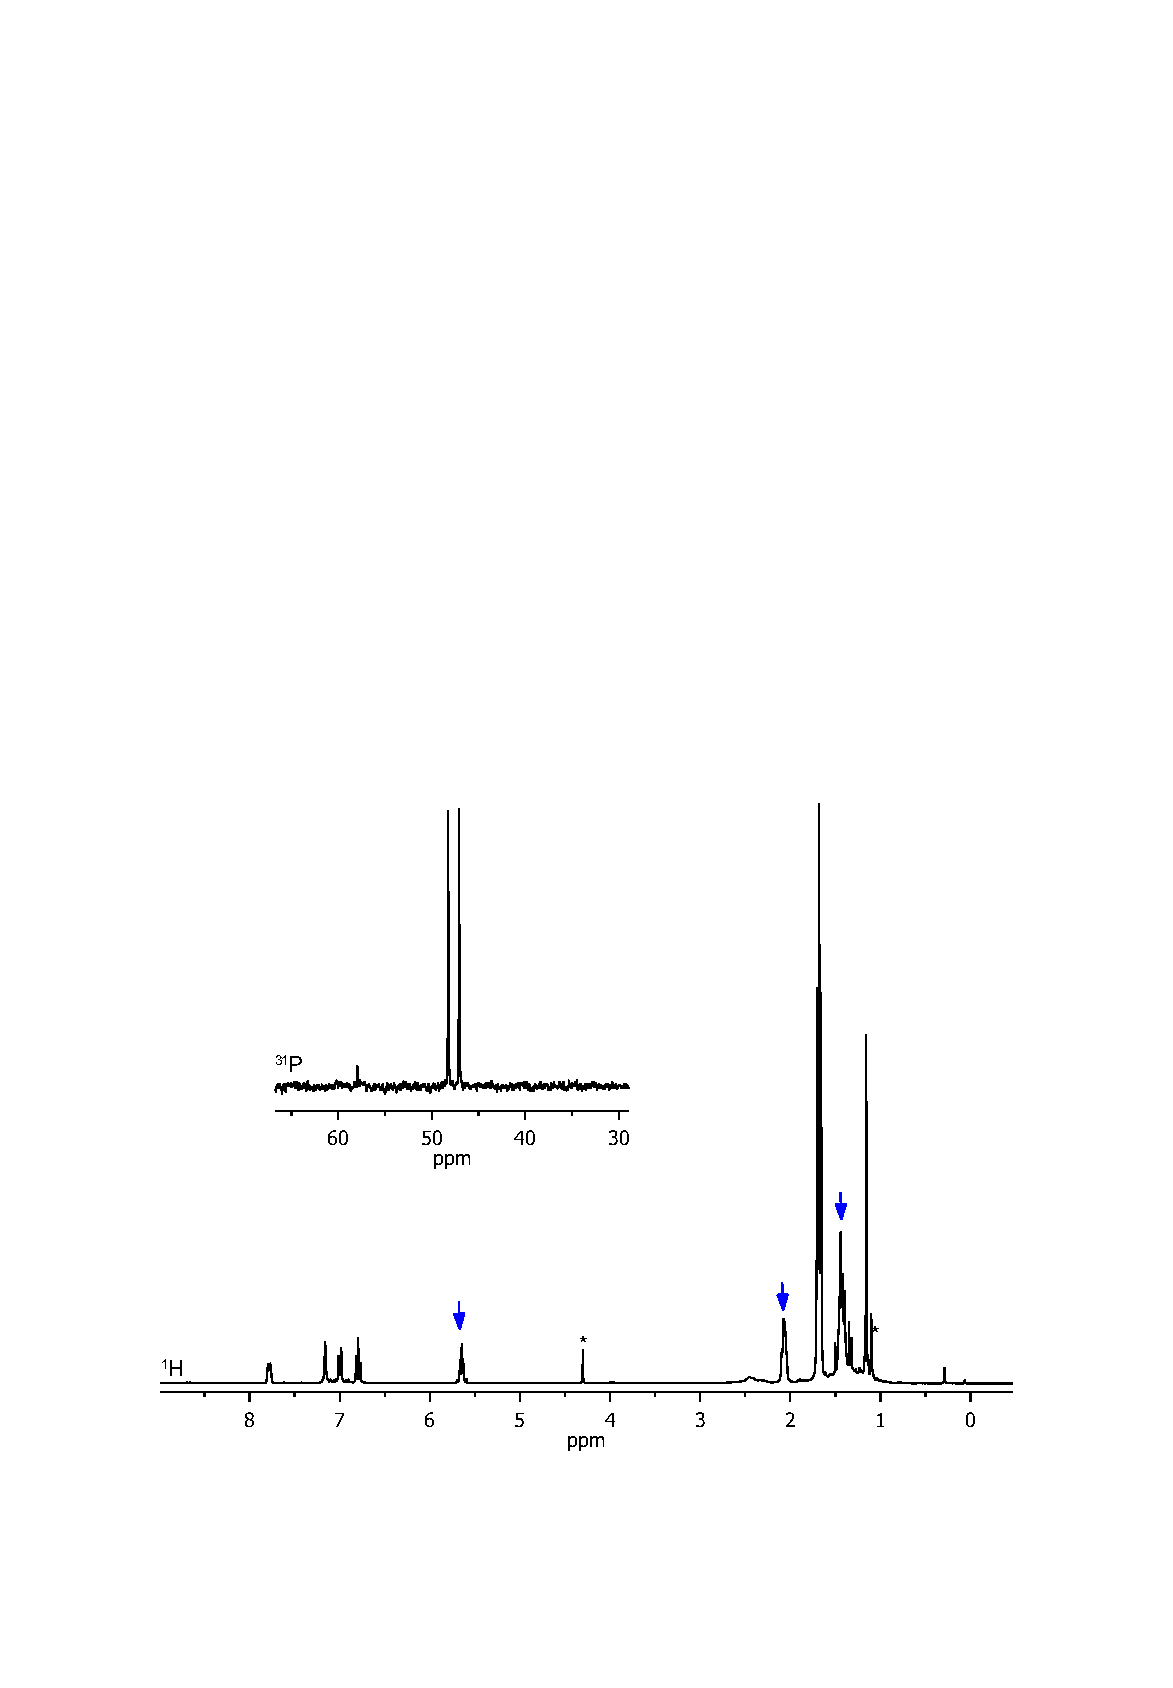
\includegraphics[trim = 2.5cm 4.0cm 2.5cm 15cm, clip]{../NMR/7004B.eps}
\caption[\phosphorus{} and \proton{} NMR spectra for [Rh(\tBuxantphos)Cl{]}]{\phosphorus{} and \proton{} NMR spectra for [Rh(\tBuxantphos)Cl]}
\vspace{0.2cm}
\label{RhClnmr}
\end{center}
\end{figure}
\vspace{0.2cm}

\begin{table}[htbp]
\caption[Selected NMR data of [Rh(\tBuxantphos)Cl{]} complexes]{Selected NMR data of [Rh(\tBuxantphos)Cl] complexes}
\vspace{1em}
\label{table:rhodiumchloride}
\small
\begin{center}
\begin{tabular}{ c c c c c c}
	\toprule{}
	~ & \multicolumn{3}{c}{\bfseries{\phosphorus}} & \multicolumn{2}{c}{\bfseries{\proton{} \emph{t}-Bu}}\\
	\cmidrule(lr){2-4} \cmidrule(lr){5-6} 
	\bfseries{Compound}&\bfseries{$\delta/$ppm}&\bfseries{$\Delta\delta/$ppm}&\bfseries{\JRhP{}$/$Hz}&\bfseries{$\delta/$ppm}&\bfseries{\J $/$Hz}\\
	\midrule{}
	SitBu	&	44.2	&	35.8	&	140.0	& 1.69	& 13.5\\
	StBu		& 	46.5	&	37.0	&	141.5	& 1.67	& 13.7\\
	CtBu		&	47.7	&	37.5	&	142.3	& 1.68	& 13.4\\
	\bottomrule{}
\end{tabular}
\end{center}
\end{table}

\begin{table}[htbp]
\caption[Chemical shift and coupling of the \emph{O}-ipso carbon when in the free ligand, [Ag(\tBuxantphos)Cl{]} and [Rh(\tBuxantphos)Cl{]} complexes]{Chemical shift and coupling of the \emph{O}-ipso carbon when in the free ligand, [Ag(\tBuxantphos)Cl] and [Rh(\tBuxantphos)Cl] complexes.}
\vspace{1em}
\label{table:oxygenbindingrh}
\small
\begin{center}
\begin{tabular}{ c c c c c c c c c}
	\toprule{}
	~&\multicolumn{2}{c}{\bfseries{Free ligand}} &\multicolumn{3}{c}{\bfseries{[Ag(\tBuxantphos)Cl]}}&\multicolumn{3}{c}{\bfseries{[Rh(\tBuxantphos)Cl]}}\\
	\cmidrule(lr){2-3} \cmidrule(lr){4-6} \cmidrule(lr){7-9}
	\bfseries{Ligand}&\bfseries{$\delta$\carbon{}$/$ppm}&\bfseries{\J{} Hz}&\bfseries{$\delta$\carbon{}$/$ppm}&\bfseries{$\Delta\delta$}&\bfseries{\J{} Hz}&\bfseries{$\delta$\carbon{}$/$ppm}&\bfseries{$\Delta\delta$}&\bfseries{\J{} Hz}\\
	\midrule{}
	\tBusixantphos	&	164.3	& 11.3	&	163.9	& -0.4	& 5.2		& 169.5	& 5.2 	& 14.4 \\
	\tButhixantphos	&	155.3	& 13.0	&	155.5	& 0.2 	& 6.6 	& 157.4	& 2.1 	&16.8 \\
	\tBuxantphos	&	155.8	& 12.0	&	156.5	& 0.7		& 6.5		& 158.9	& 3.1		& 16.3 \\
	\bottomrule{}
\end{tabular}
\end{center}
\end{table}

%A reaction occurs rapidly with all three diphosphine to form complexes \fixme{compound reference} (Scheme \ref{RhodiumI}).  These complexes have \JRhP{} coupling constants of around 142 Hz, consistent with rhodium(I).  The complexes are direct analogues of those reported for \iPrxantphos{} which has a \JRhP{} coupling constant of 142.4 Hz.\cite{Esteruelas2013}  The \tBuxantphos ligands are coordinated in a tridentate manner with the oxygen binding.  In the \carbon{} NMR spectrum this can be seen as the O-ipso carbon carbon has shifted to downfield.  For example in \tBuxantphos{} this carbon resonants at 155.8 ppm, in the complex \ce{[(tBu-xantphos)AgCl]} the carbon shifted to 156.5 although the oxygen was not binding.  In the tridentate rhodium complex this carbon has moved downfield again to 158.9 ppm.  This shift in the resonant frequency of this carbon is a result of the oxygen donating electron density to the rhodium, which in turn makes the oxygen withdraw electron density from the ipso carbons.  

\section{Reaction with Hydrogen}
\label{section:rhodiumhydride}

Rhodium complexes are well-known as homogeneous hydrogenation and hydroformylation catalysts.  Both of these processes involve the activation of molecular hydrogen at the rhodium centre.  The catalytic cycle for hydrogenation using monophosphine ligands (Scheme \ref{Hydrogenationcycle}) involves the addition of molecular hydrogen to \ce{[Rh(PR3)2Cl]} generating a rhodium dihydride, which then coordinates an alkene and hydride-migration and \chembeta-hydride elimination to generate the starting rhodium complex and the alkane, whilst in hydroformylation (Scheme \ref{Hydroformylationcycle}) the alkene in coordinated to an existing rhodium hydride complex.  Hydride migration occurs followed by carbon monoxide coordination and migratory insertion into the rhodium alkyl bond.  This is followed by the oxidative addition of dihydrogen, generating a rhodium(III) dihydride complex.  The cycle concludes by \chembeta-hydride elimination generating the aldehyde and the starting rhodium(I) complex.  Hydroformylation was the first catalytic process that the influence of the bite-angle of various xantphos complexes was studied\cite{Kranenburg1995} and has since been studied extensively both with xantphos and derivatives.\cite{Bronger2002, Bronger2003, Bronger2004, Bronger2004b, Bronger2004c, Buhling1997, Buhling1997b, Dieleman2001, Dierkes1999, Freixa2003, Goedheijt1998b, Kamer2001, Leclercq2005, Leeuwen1999, Leeuwen2000, Mora2007, Sandee1999, Silva2003, Veen1999, Veen2000, Vlugt2004, Zuidema2007, Zuidema2008, Zuidema2010}  Given the importance of the oxidative addition of molecular hydrogen for both hydrogenation and hydroformylation we investigated the reactivity of the [Rh(\tBuxantphosk)Cl] complexes with dihydrogen.  

\begin{scheme}[htbp]
\begin{center}
\vspace{0.5cm}
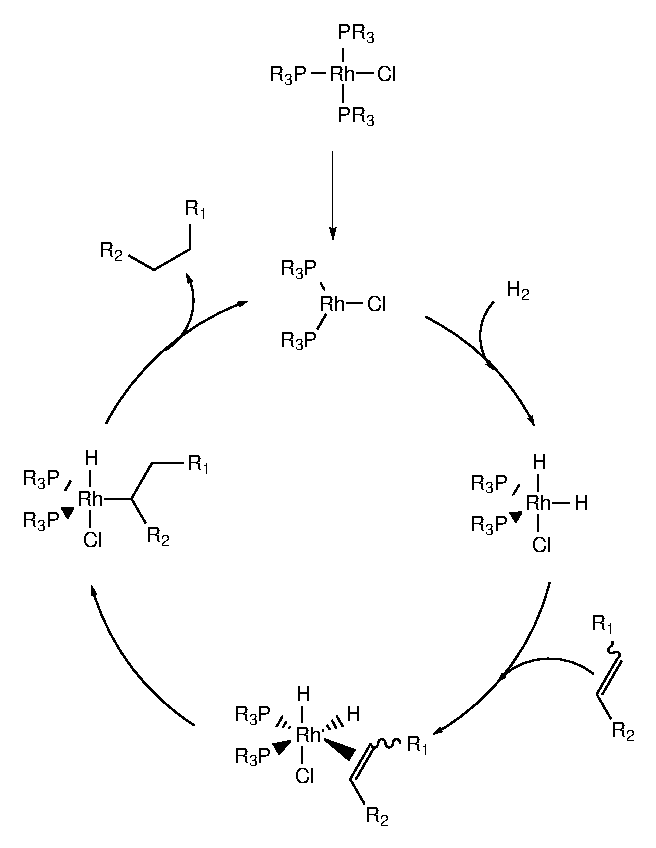
\includegraphics{../Schemes/Homogeneoushydrogenation.eps}
\caption[Catalytic cycle for homogeneous hydrogenation]{Catalytic cycle for homogeneous hydrogenation using a rhodium chloride complex with monophosphine ligands}
\vspace{0.2cm}
\label{Hydrogenationcycle}
\end{center}
\end{scheme}

\begin{scheme}[htbp]
\begin{center}
\vspace{0.5cm}
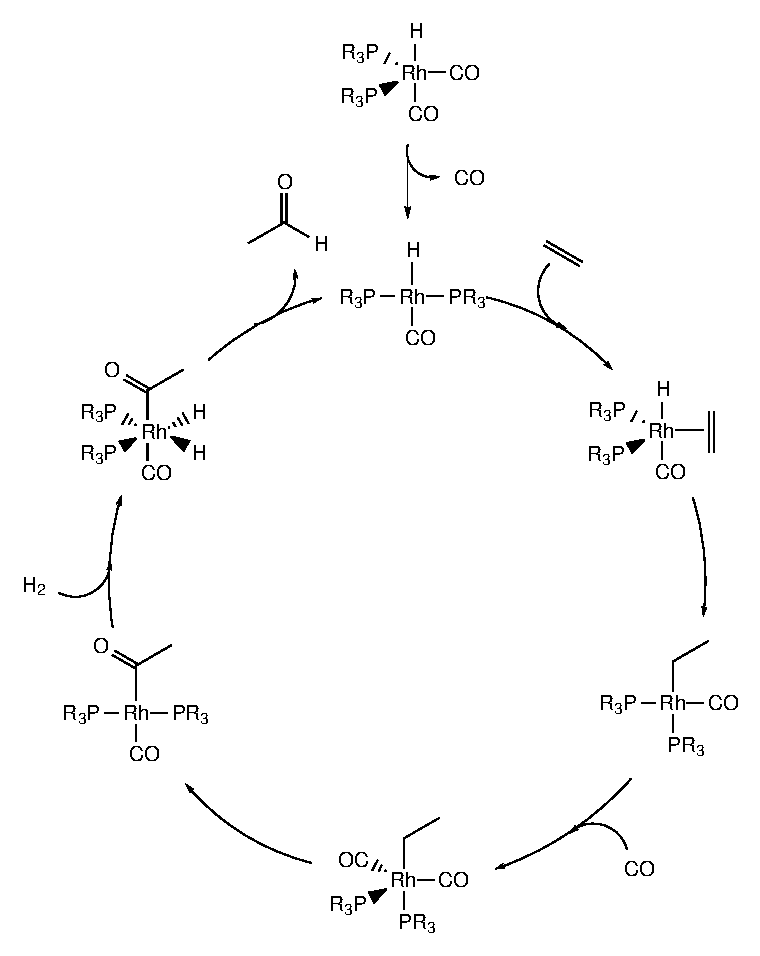
\includegraphics{../Schemes/Hydroformylationcycle.eps}
\caption[Catalytic cycle for homogeneous hydroformylation using diphosphine ligands]{Generic catalytic cycle for homogeneous hydroformylation using diphosphine ligands}
\vspace{0.2cm}
\label{Hydroformylationcycle}
\end{center}
\end{scheme}

The complexes [Rh(\tBuxantphosk)Cl] are reactive towards hydrogen, readily splitting the hydrogen to form octahedral rhodium(III) dihydride complexes (Scheme \ref{Rhodiumhydride}).  The hydrogen is split to form two different hydride environments in the product with a \cis{} arrangement.  The \tBuxantphos{} ligands retain their meridional coordination. However, as a result the two faces of the ligand are now different causing two different environments for the bridgehead methyls in both \tBusixantphos{} and \tBuxantphos{}, and the \tBu{} groups for all three \tBuxantphos{} ligands.  

\begin{scheme}[htbp]
\begin{center}
\vspace{0.5cm}
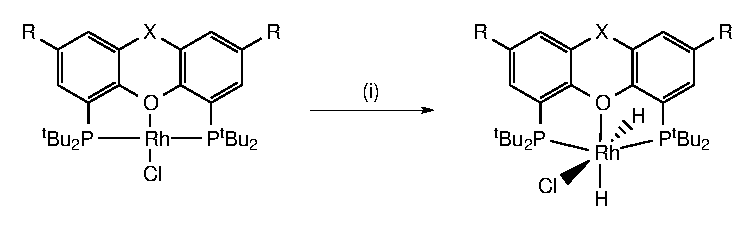
\includegraphics{../Schemes/Rhodiumhydride.eps}
\caption[Reaction of \ce{[Rh(tBu-xantphos)Cl]} with hydrogen]{Reaction of \ce{Rh(tBu-xantphos)Cl]} with hydrogen.  tBu-xantphos: R = H, X = \ce{CMe2}. tBu-thixantphos: R = Me, X = S. tBu-sixantphos: R = H, X = \ce{SiMe2}}
\vspace{0.2cm} 
\label{Rhodiumhydride}
\end{center}
\end{scheme}
\vspace{0.2cm}

Two hydride resonances are evident in the \proton{} NMR spectra occurring upfield as well defined doublets of triplets of doublets coupling to the rhodium, two phosphorus atoms and the each other (Figure \ref{rhodiumhydridenmr}, Table \ref{table:dihydrides}).  The hydride \emph{trans} to the chloride ligand (-16.92 to -17.04 ppm) shows very little change in either the chemical shift or coupling constants for the three complexes.  The hydride \trans{} to the \tBuxantphos{} oxygen (-20.51 to -21.12 ppm) shows more variance in the chemical shift and coupling.  The value \JRhH{} decreases with increasing natural bite-angle.  As the bite-angle for the \tBuxantphos{} ligand increases, the ligand will require less energy to adopt a pincer coordination mode.  This results in the larger bite-angle ligands adopting a mode closer to the ideal T-shaped pincer coordination causing a smaller Rh-O bond length.  This stronger bond in the \trans{} position results in a decreased coupling constant for the hydride ligand.  

\begin{figure}[htbp]
\begin{center}
\vspace{0.5cm}
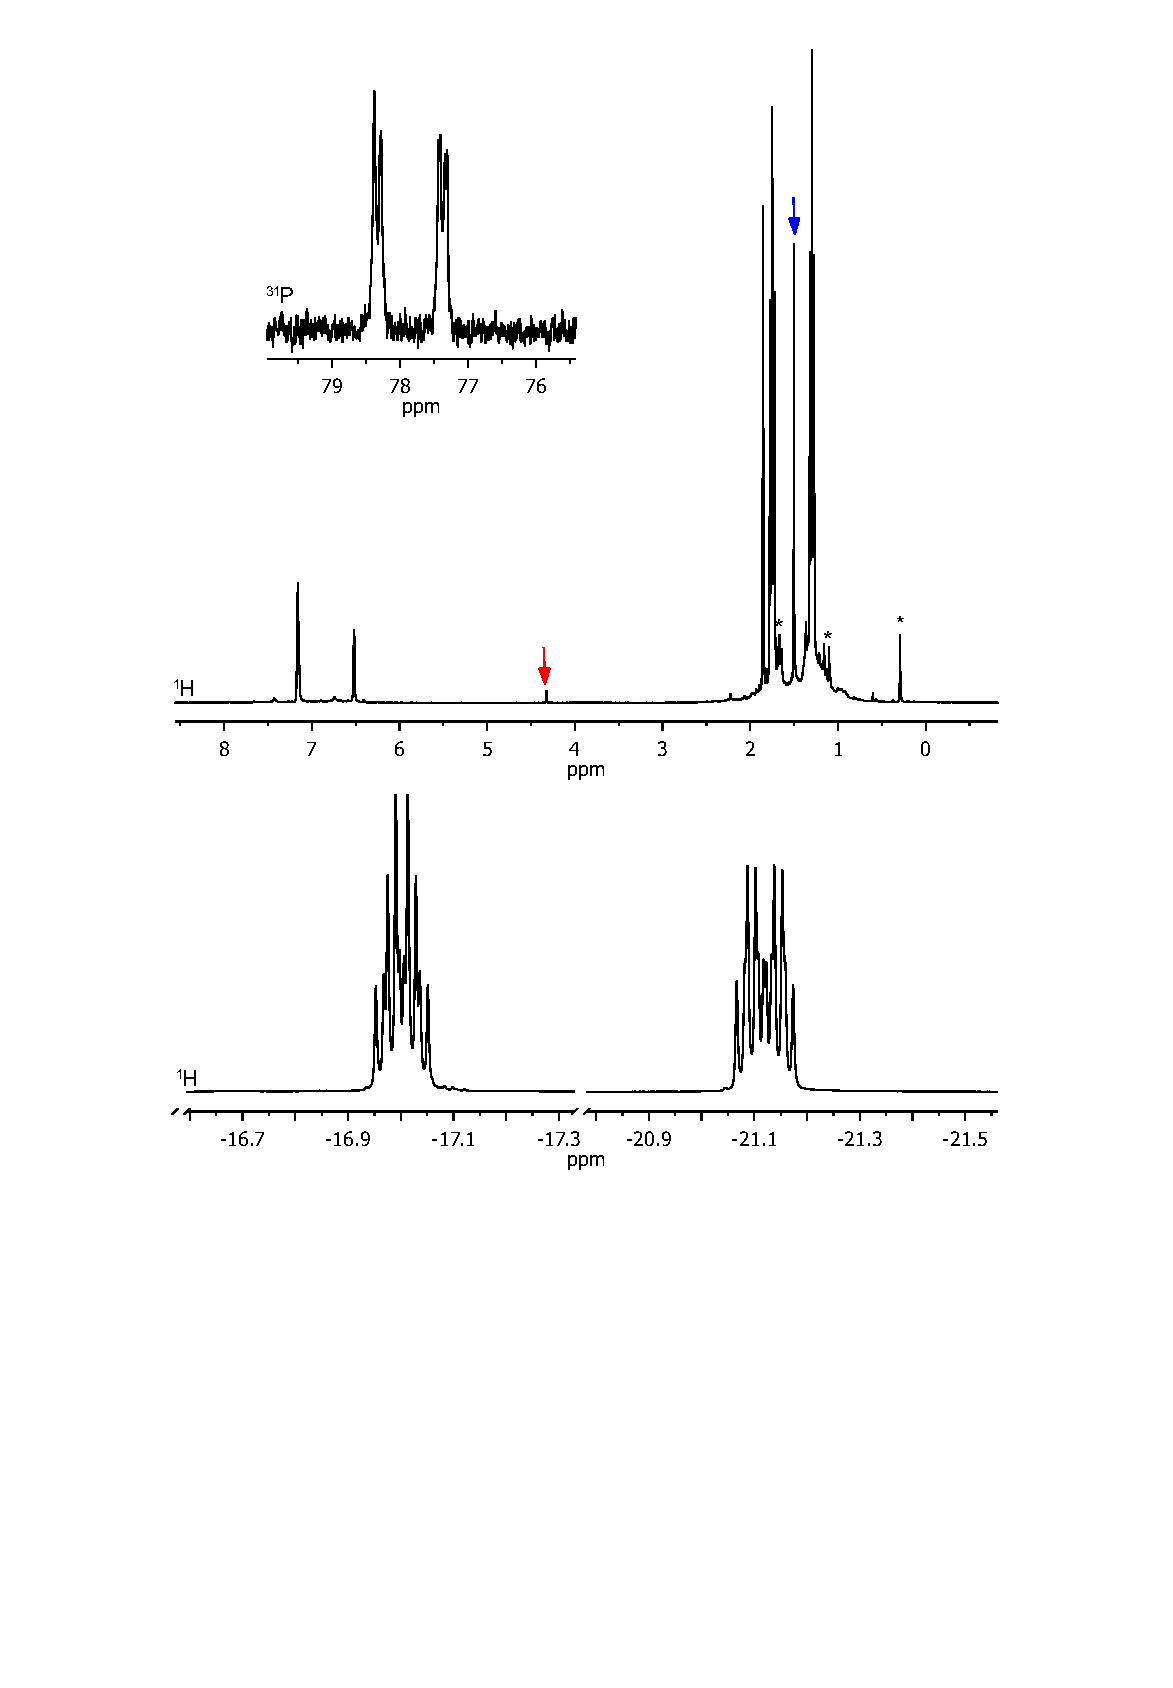
\includegraphics[trim = 2.5cm 8.5cm 2.5cm 0cm, clip]{../NMR/7006E.eps}
\caption[NMR spectra for \ce{[Rh(\tButhixantphos)Cl(H)2]}]{NMR spectra for \texorpdfstring{[Rh(\tButhixantphos)\ce{Cl(H)2]}} R.  Impurities are indicated by *, \ce{CH2Cl2} is indicated by a red arrow and cyclooctane by a blue arrow.}
\vspace{0.2cm}
\label{rhodiumhydridenmr}
\end{center}
\end{figure}
\vspace{0.2cm}

\begin{sidewaystable}
\caption[Hydride \proton{} NMR data for \ce{[Rh(\POP)Cl(H)2]}]{Hydride \proton{} NMR data for \texorpdfstring{\ce{[Rh(\POP)Cl(H)2]}}R}
\vspace{1em}
\label{table:dihydrides}
\small
\begin{center}
\begin{tabular}{c c c c c c c c c}
\toprule{}
	~~ & \multicolumn{4}{c}{\bfseries{\ce{H-} \trans-\ce{Cl-}}} & \multicolumn{4}{c}{\bfseries{\ce{H-} \trans-O}}\\
	\cmidrule(lr){2-5} \cmidrule(lr){6-9} 
	\bfseries{Diphosphine}&\bfseries{$\delta/$ppm}&\bfseries{\JRhH$/$Hz}&\bfseries{\JPH$/$Hz}&\bfseries{\JHH$/$Hz}&\bfseries{$\delta/$ppm}&\bfseries{\JRhH$/$Hz}&\bfseries{\JPH$/$Hz}&\bfseries{\JHH$/$Hz}\\
	\midrule{}
	\tBuSixantphos & -16.92 & 22.7 & 13.5 & 9.4 & -21.12 & 30.9 & 12.1 & 9.2 \\
	\tBuThixantphos & -17.00 & 22.6 & 13.5 & 9.4 & -21.13 & 30.5 & 12.4 & 9.4 \\
	\tBuXantphos & -17.04 & 22.8 & 13.4 & 9.4 & -20.51 & 28.8 & 12.2 & 9.4 \\
	\bottomrule{}
\end{tabular}
\end{center} 
\end{sidewaystable}

The \phosphorus{} NMR spectra (Figure \ref{rhodiumhydridenmr}) for the [Rh(\tBuxantphosk)\ce{(H)2Cl]} complexes each display a single resonance downfield relative to the starting [Rh(\tBuxantphosk)Cl] complexes as a doublet of doublets with some further coupling evident.  Although \phosphorus{} NMR is \proton{} decoupled the decoupler is unable to decouple resonances that are so far outside the typical \proton{} range (-2 to 15 ppm) resulting in the residual coupling.  The value of \JRhP{} has decreased by 23.7-25.3 Hz to 116.1-117.8 Hz consistent with a change in the oxidation state of the rhodium centre from Rh(I) to Rh(III).  Consistent with the proposed geometry, the \proton{} NMR spectra also display two signals for the \tBu{} protons, both appearing as virtual triplets indicating the \trans{} coordination of the phosphorus atoms.  Two signals were also observed in the \proton{} NMR spectra for the bridgehead methyls in [Rh(\tBuxantphosk\ce{)(H)2Cl]} and [Rh(\tBusixantphosk\ce{)(H)2Cl]}, again consistent with the proposed structure.  

The [Rh(\tBuxantphosk\ce{)(H)2Cl]} complexes are similar to previously reported dihydride complexes of \iPrxantphos{}\cite{Esteruelas2013, Esteruelas2013b} and \Phxantphos{}\cite{Dallanegra2012, Johnson2013, Pawley2010}.   In these cases the hydride \trans{} to the oxygen atom was located in the \proton{} NMR between -22.19 and -19.00 ppm with a rhodium coupling constant of 27.0 - 33.8 Hz.  The \proton{} NMR signals for the hydride in the [Rh(\tBuxantphosk\ce{)(H)2Cl]} complexes are encompassed within these ranges (Table \ref{table:dihydrides}).  For the reported \tBuxantphos{} complexes the \phosphorus{} chemical shift is 77.8-79.0 ppm with \JRhP{} = 116.1-117.8 Hz.  In comparison the literature complexes appear at 36.9-45.4 ppm and \JRhP{} = 114-121 for \Phxantphos{} and 64.8-67.2 ppm and 113-114 Hz for \iPrxantphos{}.  The coupling constants are consistent for the complexes, and although the absolute chemical shift varies significantly, the change in chemical shift from the [Rh(I)(POP)Cl] complexes is consistent (28.7-31.1 ppm for \iPrxantphos{} compared to 31.3-34.0 ppm for \tBuxantphos{}, [Rh(\Phxantphos)Cl] has not been reported in the literature).  

In some cases with \Phxantphos{} \fixme{the complexes (define which complexes)} were reportedly only stable under a hydrogen atmosphere,\cite{Johnson2013, Dallanegra2012} however, in the case of \tBuxantphos{} the complexes were able to be placed under vacuum overnight with no evidence for loss of hydrogen.  This difference is likely the result of the different electronics between \tBuxantphos{} and \Phxantphos{}.  The electron donating nature of the \tBu{} groups on \tBuxantphos{} enhances electron donation from the rhodium centre into the $\sigma$* orbital of a dihydrogen ligand, thus favouring oxidative addition and the formation of two discrete hydrides.  As the \Phxantphos{} has two electron withdrawing phenyl substituents on each phosphorus atom together with the aromatic backbone of the ligand this will have less back-bonding and thus less of a barrier towards the reformation of a dihydrogen ligand which could dissociate under vacuum.

The synthesis of [Rh(\tBuxantphosk)Cl] from \ce{[Rh(COE)2Cl]2} generates free cyclooctene as a by-product.  This reaction mixture was used without further purification to determine the potential for the [Rh(\tBuxantphosk)Cl] complexes to act as hydrogenation catalysts.  Hydrogen gas was bubbled through a mixture of [Rh(\tBuxantphosk)Cl] and cyclooctene for 10 minutes before the reaction was sealed and allowed to proceed at room temperature.  After \fixme{some amount of time} no evidence for cyclooctene was observed by \proton{} NMR spectroscopy in the reaction mixture and a peak for cyclooctane was apparent (Figure \ref{rhodiumhydridenmr}).  While further work to determine the activity of these complexes needs to be performed, this result indicates the potential for the [Rh(\tBuxantphosk)Cl] to act as precatalyts for hydrogenation of alkenes.  

%The hydrides appear as two signals in the \proton{} NMR spectrum upfield at -17.12 ppm and -20.54 ppm (dtd, \JRhH = 28.7, \JPH = 12.1, \JHH = 9.1) \fixme{give coupling constants} as doublets of triplets of doublets coupling to the rhodium, two phosphorus' and the other hydride.  \fixme{put in a picture of this because it's kind of awesome}  This downfield shift of the O-ipso carbon is retained at \fixme{value} indicating that the tridentate coordination of the xantphos ligand is retained.  This reaction appears to be reversible an equilibrium such that at 1 atm of hydrogen a ratio of \fixme{value} between the two species is observed.  Over time as the hydrogen dissipates out of the NMR tube the reaction returns to starting material.  In addition this complex does convert to the unknown rhodium(III) species over time.  This is likely due to the hydrogen dissipating resulting in return to the rhodium(I) species which then reacts to the unknown rhodium(III) complex.

\subsection{Protonation of \texorpdfstring{[Rh(\tButhixantphos)\ce{Cl(H)2]}} R Complexes}

In order for molecular hydrogen to oxidatively add to the rhodium centre it must first coordination as an \hapto{2}-dihydrogen ligand.  Since their discovery by Kubas in 1984\cite{Kubas1984} several hundred dihydrogen complexes have been reported.\cite{McGrady2003}  However, despite their implication as intermediates in a number of catalytic processes including hydrogenation and hydroformylation rhodium complexes of \hapto{2}-dihydrogen are surprisingly rare.  Dihydrogen coordinates to a metal centre by donation from the H-H $\sigma$-bonding orbital to the metal centre and back-donation from the metal into the H-H $\sigma*$ orbital.  Thus complexes of the late transition metals, especially those with strongly electron donating phosphines such as \tBuxantphos{} result in the oxidative addition of hydrogen rather than coordination as a dihydrogen moiety.  However, dihydrogen complexes can also be synthesised by protonation of preformed metal hydride complexes.  First reported as a synthetic method by Crabtree and coworkers in 1986\cite{Crabtree1986} this method has since been used to create numerous dihydrogen complexes\cite{Janak2004, Oldham1997, Pons2004, Heinekey1993}.

%The rhodium dihydride complexes are stable and do not need to be stored under a hydrogen atmosphere, showing no degradation after storing under argon.  These complexes are not air-stable however as will be discussed in Section \ref{section:rhodium oxygen}. 

As previously discussed the addition of molecular hydrogen to the [Rh(\tBuxantphosk)Cl] complexes resulted in cleavage of the H-H bond and formation of the dihydride complexes [Rh(\tBuxantphosk)\ce{(H)2Cl]}.  These dihydride complexes were treated with one equivalent of the strong acid, \ce{CH2(SO2CF3)2}, or \ce{HBF4.OEt2}.  With either acid and all three \tBuxantphos{} ligands the \phosphorus{} NMR spectra showed negligible change (Table \ref{table:dihydrogen}).  In the \proton{} NMR spectrum the aromatic signals are unchanged.  However, the \tBu{} resonances had changed from two virtual triplets to a broad singlet.  A similar effect was observed for the NMR signals for the bridgehead methyls in \tBuxantphos{} and \tBusixantphos{}.  The methyl groups on the backbone of \tButhixantphos{} remained as a singlet as they are already equivalent in the dihydride complexes.  The resonances attributed to the hydride signals in [Rh(\tBuxantphosk)\ce{(H)2Cl]} were well-resolved doublets of triplets of doublets.  Upon protonation these were replaced by two broad resonances with essentially no change in chemical shift.  When protonation was carried out with \ce{CH2(SO2CF3)2} the \fluorine{} NMR showed a singlet peak at between -76.2 and -76.4 ppm indicative of the non-coordinated \ce{CH(SO2CF3)2-} anion.

The NMR data from the protonation of [Rh(\tBuxantphosk)\ce{(H)2Cl}] with \ce{CH2(SO2CF3)2} shows very little change except for some broadening of parts of the spectrum.  From this we propose that an equilibrium state is achieved between a number of different species however, this equilibrium heavily favours the initial dihydride complex (Scheme \ref{rhodiumdihydrogen}).  Dihydrogen complexes with additional hydride ligands frequently display exchange of the dihydrogen and hydride sites in the complex.\cite{Crabtree1986, Findlater2012, Hamilton1988, Heinekey1993, Janak2004}  

\begin{scheme}[htbp]
\begin{center}
\vspace{0.5cm}
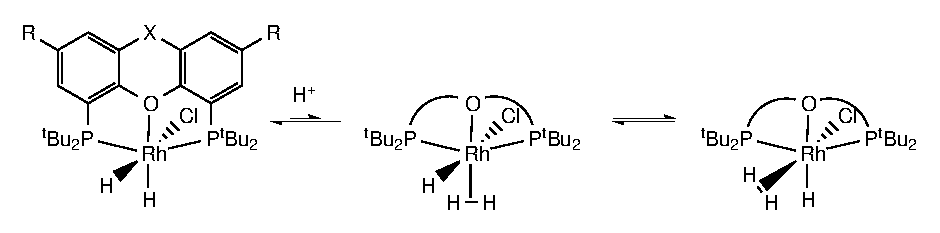
\includegraphics{../Schemes/Rhodiumdihydrogen.eps}
\caption[Dynamic behaviour of rhodium dihydrogen complexes]{Dynamic behaviour of rhodium dihydrogen complexes}
\vspace{0.2cm}
\label{rhodiumdihydrogen}
\end{center}
\end{scheme}
\vspace{0.2cm}

When \ce{HBF4.OEt2} was used instead of \ce{CH2(SO2CF3)2} a peak for the free \ce{BF4-} counterion was not observed (expected =151 ppm\cite{Feller2007})  Instead the \fluorine{} NMR spectrum showed a number of peaks between -142 and -156 ppm, some of these peaks were of similar intensities indicating the possibility of coupling to a rhodium centre.  In this case the \proton{} NMR is very similar to that for the reaction with \ce{CH2(SO2CF3)2} indicating that an equilibrium has likely been established.  In this case however, once the chloride has dissociated a \ce{BF4-} ligand may coordinate in its place resulting in the mixture of species observed in the \fluorine{} NMR spectrum.   However, rhodium complexes with monodentate \ce{BF4-} ligands coordinated through one of the fluorine atoms generally come between -164 and -160 ppm in the \fluorine{} NMR spectrum.\cite{Feller2007, Salem2006, Salem2008, Gandelman2003}

\fixme{write about mass spec results}

%Negligible difference was observed in the \phosphorus{} NMR spectrum and the aromatic resonances of the \proton{} and \carbon{} NMR spectra (Table \ref{table:dihydrogen}).  However, the resonances for the \tBu{} and hydridic protons and carbons are very broad, coalescing to a single broad peak for the \tBu{} protons and two broad peaks for the \tBu{} carbons.  The hydridic protons appear in the same position as the dihydride however the well-resolved doublets-of-triplets-of-doublets have been replaced by two very broad singlets. 

\begin{table}[htbp]
\caption[Selected NMR data of rhodium dihydride and dihydrogen complexes]{Selected NMR data of rhodium dihydride and dihydrogen complexes} 
\vspace{1em}
\label{table:dihydrogen}
\small
\begin{center}
\begin{tabular}{ c c c c c}
	\toprule{}
	~~ & \multicolumn{2}{c}{\bfseries{Dihydride}} & \multicolumn{2}{c}{\bfseries{Protonated}}\\
	\cmidrule(lr){2-3} \cmidrule(lr){4-5}
	\bfseries{Diphosphine}&\bfseries{$\delta$\phosphorus{}$/$ppm}&\bfseries{\JRhP$/$Hz}&\bfseries{$\delta$\phosphorus{}$/$ppm}&\bfseries{\JRhP$/$Hz}\\
	\midrule{}
	SitBu	&	78.2	&	116.1	&	78.1		&	115.6\\
	StBu		& 	77.8	&	117.8	&	77.7		&	115.7\\
	CtBu		&	79.0	&	117.0	&	78.9		&	115.6\\
	\bottomrule{}
\end{tabular}
\end{center}
\end{table}


\section{Rhodium Carbonyl Complexes}

Metal carbonyl complexes are some of the most well-studied complexes for a number of reasons.  Metal carbonyls are used in a number of different catalytic processes including hydroformylation, hydroesterification and hydrocarboxylation to introduce oxygen functionality.  These reactions are of great synthetic importance and numerous industrial examples are known such as the conversion of a benzylic alcohol to a carboxylic acid using a palladium catalyst in the synthesis of ibuprofen.\cite{Kjonaas2011} and the hydroformylation of 1,3-butadiene to adipaldehyde an intermediate for producing caprolactam and hexamethylene-1,6-diamine (HMDA) both key monomers for nylon-6.6 and nylon-6 manufacture.\cite{Franke2012}  These catalytic processes involve the terminal coordination of the carbonyl to the metal centre.  However carbonyls can also act as bridging ligands either solely through the carbon atom, or involving the oxygen as a terminal ligand or the side-on \hapto{2} mode involving the $\pi$-system.  

Transition metal carbonyl complexes have also long been studied to investigate the electronic influence of other ligands.  The stretching frequency of the \ce{C#O} bond is a good measure of the electronic environment as carbonyl ligands are strong $\pi$-acceptor ligands, meaning that the metal centre will donate electron density into the $\pi*$-orbital.  This in turn weakens the \ce{C#O} and results in a shift of the infrared \ce{C#O} stretch to lower frequency.  The degree to which the back-bonding occurs is related to the nature of the metal centre and the other ligands.  As such a number of series exist where this stretch has been used to quantify the electron donor capabilities of various ligands.  These include the well-known Tolman Electronic Parameter using \ce{[Ni(CO)3L]} complexes,\cite{Tolman1977} \ce{[Mo(CO)5L]} and \ce{[Rh(CO)ClL2]} series,\cite{Banger2009}  although other methods are utilised such as the phosphine selenide coupling constants (see Section \ref{section:selenides}) and the \JPtP{} coupling in \cis-\ce{[PtCl2L2]} complexes.\cite{Banger2009}

The typical method for producing rhodium carbonyl complexes is to react the free phosphine or diphosphine ligand with either the chloro-bridged dimer, \ce{[Rh(CO)2Cl]2}, or by reaction with a chloro-bridged rhodium alkene dimer such as \ce{[Rh(C2H4)2Cl]2} or \ce{[Rh(COE)2Cl]2} while under an atmosphere of carbon monoxide.  The reaction is then worked up either in the air or under inert atmosphere and in the majority of cases the product is \trans-\ce{[Rh(CO)(PP)Cl]} where PP is either two monophosphine ligands or a \trans-spanning diphosphine.  Using smaller bite-angle diphosphine ligands results in the \cis{} isomer.  

The reactivity of the [Rh(\tBuxantphosk)Cl] complexes towards carbon monoxide was investigated on an NMR scale by bubbling CO through an sample of the complex for 10 mins before sealing the NMR tube with a J. Young tap.  Immediate NMR analysis of these samples showed the reaction was complete with no evidence for starting material and a single product formed.  A colour change was observed changing from the dark brown starting material to yellow (\tBusixantphos) or orange (\tButhixantphos{} and \tBuxantphos).

The NMR spectra for the three resulting products show some differences.  The \proton{} and \carbon{} NMR spectra for the reaction of [Rh(\tButhixantphosk)Cl] with CO is broad, possibly indicating dynamic behaviour.  However the \phosphorus{} NMR spectrum shows only slight broadening.  However, the spectra for the reaction of [Rh(\tBusixantphosk)Cl] and [Rh(\tBuxantphosk)] with CO are both well-resolved (Figure \ref{Rhcarbonylnmr} shows a selection of the NMR spectra for the \tBuxantphos{} complex).

\begin{figure}[htbp]
\begin{center}
\vspace{0.5cm}
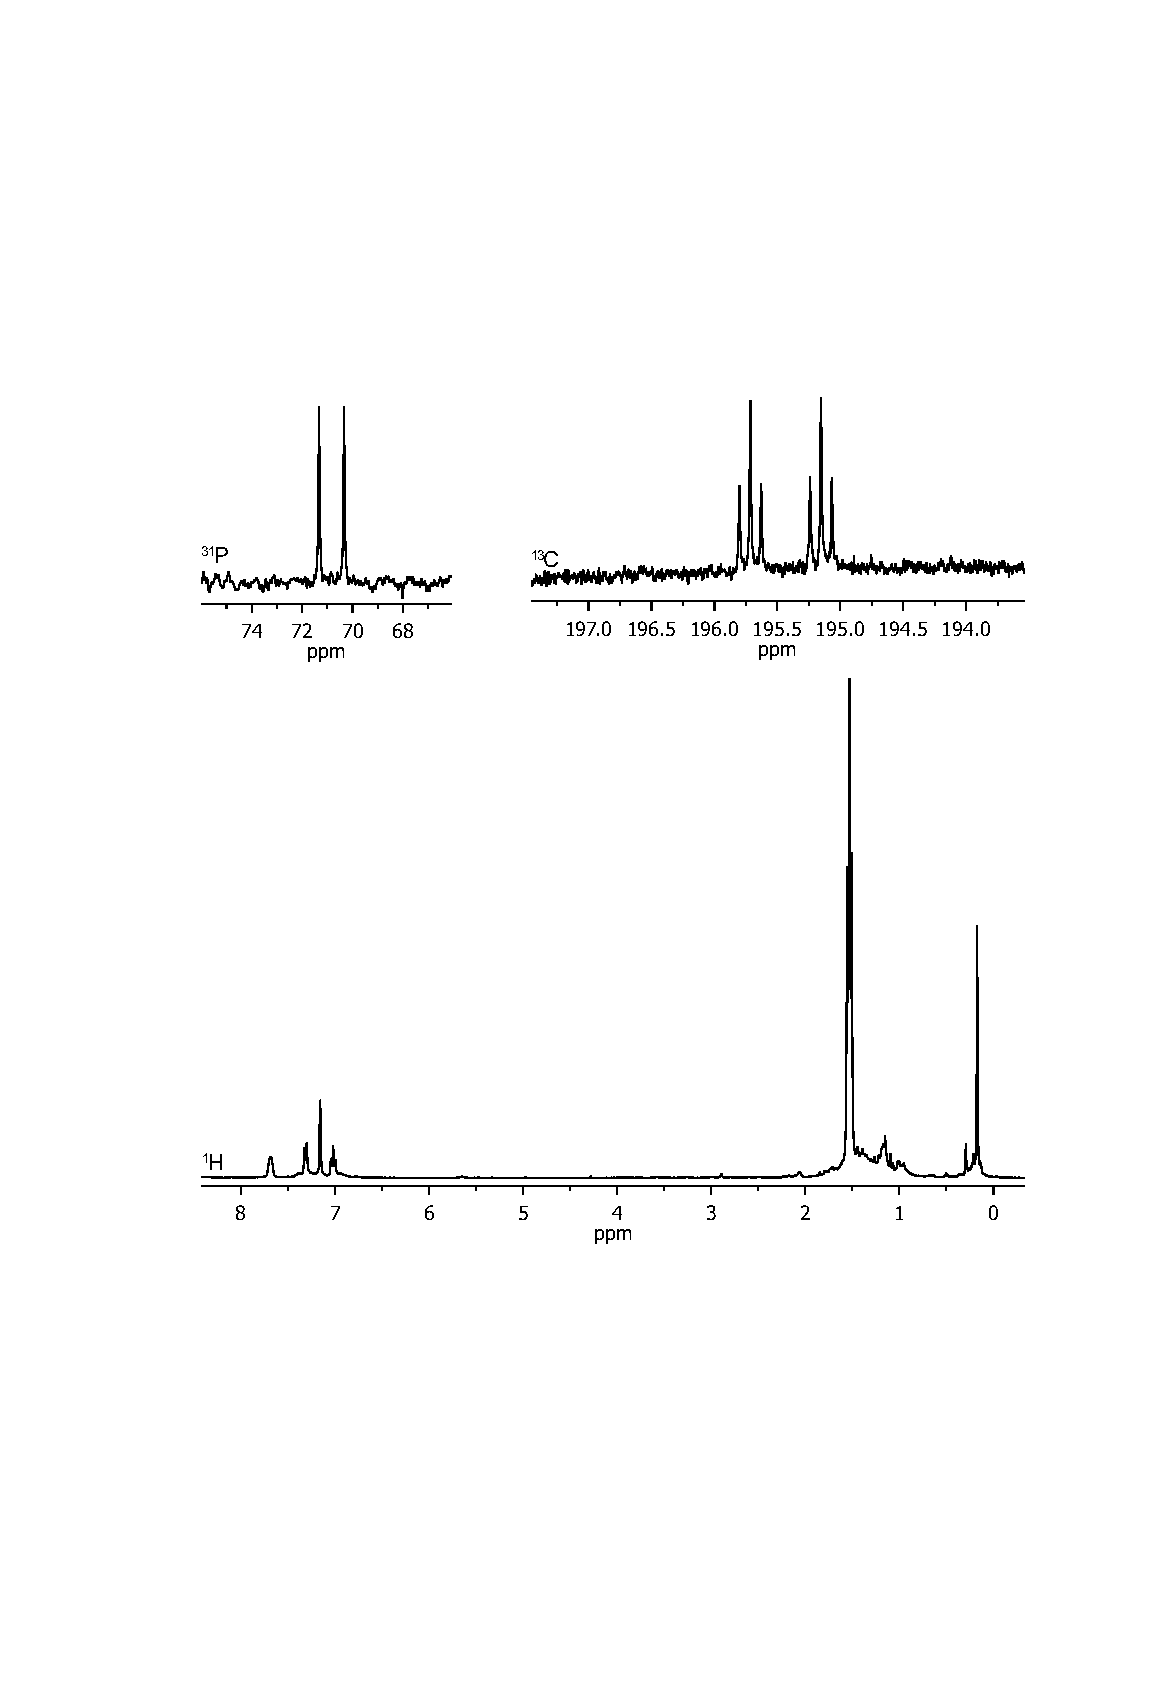
\includegraphics[trim = 2.5cm 7.2cm 2.5cm 5.0cm, clip]{../NMR/7017.eps}
\caption[\phosphorus{} and \proton{} NMR spectra for [Rh(\tBuxantphos)Cl{]}(CO)2]{\phosphorus{} and \proton{} NMR spectra for \ce{[Rh(\tBuxantphos)Cl(CO)2]} in \ce{C6D6}}
\vspace{0.2cm}
\label{Rhcarbonylnmr}
\end{center}
\end{figure}
\vspace{0.2cm}

In all cases the \phosphorus{} NMR spectrum showed a single peak at 69.3 - 71.6 ppm, split into a doublet by rhodium coupling of 120.0 - 122.2 Hz (Table \ref{table:rhodiumcarbonyl}).  These are shifted downfield relative to the [Rh(\tBuxantphosk)Cl] starting material, to a similar place as the [Rh(\tBuxantphosk)\ce{(H)2Cl]} indicating the presence of strongly coordinating ligands (like CO).  The value of \JRhP{} has decreased from the starting [Rh(\tBuxantphosk)Cl] complexes from 140-142.3 Hz to 120.0-122.2 Hz.

\begin{table}[htbp]
\caption[Selected NMR data of [Rh(\tBuxantphos)\ce{(CO)2Cl}{]} complexes]{Selected NMR data of [Rh(\tBuxantphos)\ce{(CO)2Cl]} complexes}
\vspace{1em}
\label{table:rhodiumcarbonyl}
\small
\begin{center}
\begin{tabular}{ c c c c c c c}
	\toprule{}
	~ & \multicolumn{3}{c}{\bfseries{\phosphorus}} & \multicolumn{3}{c}{\bfseries{\carbon{} CO}} \\
	\cmidrule(lr){2-4} \cmidrule(lr){5-7}
	\bfseries{Ligand}&\bfseries{$\delta/$ppm}&\bfseries{$\Delta\delta$ ppm}&\bfseries{\JRhP{}$/$Hz}&\bfseries{$\delta/$ppm}&\bfseries{\JRhC $/$Hz}&\bfseries{\JPC $/$Hz}\\
	\midrule{}
	\tBusixantphos	&	70.8	&	26.6 & 120.0	&	195.5	& 84.4	& 13.0\\
	\tButhixantphos	& 	69.3	&	22.8	& 122.2	&	not observed	& 	& \\
	\tBuxantphos	&	71.6	&	23.9	& 120.0	&	194.9	& 84.4	& 12.4\\
	\bottomrule{}
\end{tabular}
\end{center}
\end{table}

%\fixme{talk about the coupling constant relative to other rhodium carbonyl complexes}

The NMR spectra for the products indicates a high level of symmetry in the resulting complexes.  
In the \proton{} NMR spectra a single peak was observed for the \tBu{} groups and a single singlet was observed for the methyl groups.  Half the expected number of signals for the aromatic protons were observed.  This indicates that two mirror planes exist, parallel to the backbone of the ligand and perpendicular to it (running through the oxygen and other bridging atom).  For \tBusixantphos{} and \tBuxantphos{} the \tBu{} groups appear as a virtual triplet indicating a \trans{} or pseudo \trans{} coordination geometry.  For \tButhixantphos{} the \tBu{} resonance displays some broadening resulting in a singlet resonance.

The \carbon{} NMR spectra are also consistent with a highly symmetric product.  For \tBusixantphos{} and \tButhixantphos{} only 9 peaks due to the ligand were present, while for \tBuxantphos{} the 10 peaks were present (one extra due to the bridgehead carbon).  In the case of \tButhixantphos{} all of these peaks were broad except two which can be attributed to the methyl groups and the aromatic carbon they are attached to, indicating that these carbons are unaffected by the dynamic process.  

Although the reaction was carried out with natural abundance CO, in the \carbon{} NMR spectra for \tBusixantphos{} and \tBuxantphos{} a peak was apparent for the coordinated carbonyl (Table \ref{table:rhodiumcarbonyl} and Figure \ref{Rhcarbonylnmr}).  This peak occurs at 195.5 ppm for \tBusixantphos{} and 194.9 ppm for \tBuxantphos{} as a well-resolved doublet of triplets indicating coupling to rhodium (\JRhC{} = 84.4 Hz for both) and two phosphorus atoms (\JPC{} = 13.0 and 12.4 Hz for \tBusixantphos{} and \tBuxantphos{} respectively).  The \JRhC{} coupling constants are both 84.4 Hz.  As coupling constants are heavily influenced by the ligand in the \trans{} position it is likely that the carbonyl is in the same environment in both complexes likely a \cis{} position relative to the phosphorus atoms as a \trans{} coordination to either the phosphorus or oxygen donor atoms would likely result in a change in the value of \JRhC{}.  However, in this particular case the \phosphorus{} NMR spectrum for the \tBusixantphos{} and \tBuxantphos{} complexes display identical \JRhP{} values.  

 %\fixme{talk about the position of this peak}

There are a number of different possible products for the reaction of the [Rh(\tBuxantphosk)Cl] complexes with carbon monoxide due to the ability of rhodium(I) to form both square-planar and trigonal bipyramidal structures combined with the potential hemilability of the \tBuxantphos{} oxygen resulting in a \dento{}PP\textprime{} bonding geometry.  In addition it is possible for either one or two carbonyl ligands to coordinate displacing either the oxygen or the chloride ligand.  The number of possibilities is decreased by the inability for the \tBuxantphos{} ligands to coordinate in a \cis{} geometry on square planar centres (\fixme{reference to platinum section}) thus also eliminating trigonal bipyramidal products with the \tBuxantphos{} complex coordinated in an \dento{}P,P\textprime{} axial-equitorial position.  Possible products from the reaction are outlined in Figure \ref{RhCOpossibilities}.

\begin{figure}[htb]
\begin{center}
\vspace{0.5cm}
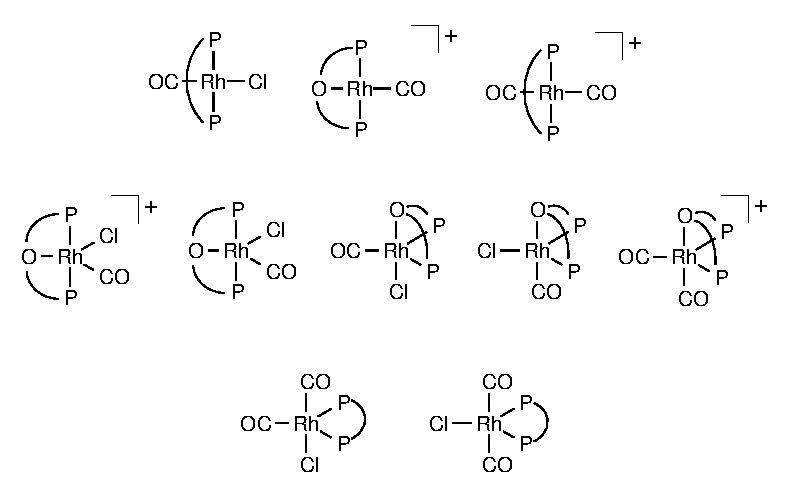
\includegraphics{../Figures/RhCOpossibilities.eps}
\caption[Possible products from reaction of \texorpdfstring{[Rh(\tBuxantphosk)Cl{]} complexes with CO} R]{Possible products from reaction of \texorpdfstring{[Rh(\tBuxantphosk)Cl] complexes with CO} R.  First row: tetrahedral complexes, second row: trigonal bipyramidal complexes with \dento{}P,O,P\textprime{} \tBuxantphos{}, and third row: trigonal bipyramidal complexes with \dento{}P,P\textprime{} \tBuxantphos{} ligands}
\vspace{0.2cm}
\label{RhCOpossibilities}
\end{center}
\end{figure}
\vspace{0.2cm}

The majority of the possible structures outlined in Figure \ref{RhCOpossibilities} can be discounted as they do no meet the symmetry requirements determined from the NMR spectra.  The only two complexes are the square planar complexes, [Rh(\tBuxantphosk)CO]Cl and [Rh\tBuxantphos\dento{}P,P\textprime\ce{(CO)2]Cl}, and the trigonal bipyramidal complex \trans-[Rh(\tBuxantphos\dento{}P,P\textprime\ce{(CO)2Cl]} \fixme{consider making this the full (TBPY name)}.  The mass spectrometry for the product from the reaction of [Rh(\tBuxantphos)Cl] with CO show a single major ion cluster.  This cluster only differs for the three ligands due to the differences in the ligand structure.  The cluster is consistent with a [Rh(\tBuxantphos)\ce{(CO)]+} ion in both mass/charge ratio and the isotopic distribution.  While this supports the formulation of the product as a monocarbonyl entity this ion cluster could result from any of the possible structures given in Figure \ref{RhCOpossibilities} as mass spectrometry is performed under high vacuum which may result in loss of CO from the dicarbonyl structures and ionisation by loss of chloride ligands is very common for coordination complexes.

As previously discussed (Section \ref{section:rhodiumchloride}) the position of the \emph{O}-ipso carbon peak in the \carbon{} NMR spectra for \tBuxantphos{} complexes can be used as a guide for the bonding mode of the ligand.  A peak for the  \emph{O}-ipso carbon that has not shifted significantly from the \emph{O}-ipso carbon peak for the free ligand is indicative of a \dento{}P,P\textprime coordination, while a peak shifted downfield by more than 2.0 ppm is indicative of a \dento{}P,O,P\textprime coordination.   The products from this reaction show very little change in the position of the \emph{O}-ipso peak compared to the free ligand (Table \ref{table:RhcarbonylOpeak}).  Thus indicating that the  coordination mode of the three \tBuxantphos{} ligands in these carbonyl complexes is most likely to be a bidentate \dento{}P,P\textprime mode.

\begin{table}[htbp]
\caption[Chemical shift and coupling for the \emph{O}-ipso carbon in \tBuxantphos{}, [Rh(\tBuxantphos)Cl{]} and carbonyl complexes]{Chemical shift and coupling for the \emph{O}-ipso carbon in \tBuxantphos{}, [Rh(\tBuxantphos)Cl{]} and carbonyl complexes.}
\vspace{1em}
\label{table:RhcarbonylOpeak}
\small
\begin{center}
\begin{tabular}{ c c c c c c c c c}
	\toprule{}
~&\multicolumn{2}{c}{\bfseries{Free ligand}} &\multicolumn{3}{c}{\bfseries{[Rh(\tBuxantphos)Cl]}}&\multicolumn{3}{c}{\bfseries{[Rh(\tBuxantphos)\ce{(CO)2Cl]}}}\\  
	\cmidrule(lr){2-3} \cmidrule(lr){4-6} \cmidrule(lr){7-9}
	\bfseries{Ligand}&\bfseries{$\delta$\carbon{}$/$ppm}&\bfseries{\J{} Hz}&\bfseries{$\delta$\carbon{}$/$ppm}&\bfseries{$\Delta\delta$}&\bfseries{\J{} Hz}&\bfseries{$\delta$\carbon{}$/$ppm}&\bfseries{$\Delta\delta$}&\bfseries{\J{} Hz}\\
	\midrule{}
	\tBusixantphos	&	164.3	& 11.3	&	169.5	& 5.2		& 14.4	& 164.3	& 0.0 	& 8.1 \\
	\tButhixantphos	&	155.3	& 13.0	&	157.4	& 2.1 	& 16.8 	& 154.9	& -0.4 &n.o. \\
	\tBuxantphos	&	155.8	& 12.0	&	158.9	& 3.1		& 16.3	& 155.6	& -0.2	& 10.4 \\
	\bottomrule{}
\end{tabular}
\end{center}
\end{table}
\fixme{make some note about the delta delta values being from the free ligand}

The two possible square planar complexes are positively charged.  As such, we would expect them not to be soluble in \ce{C6D6}.  However, the product of this reaction remains in a \ce{C6D6} solution with no signs of precipitation over a period of several weeks.  This supports the formation of the product as \trans-[Rh(\tBuxantphos)\ce{(CO)2}Cl].  Rhodium dicarbonyl complexes are typically only stable below room temperature and under an atmosphere of carbon monoxide, readily losing CO under vacuum.\cite{Sanger1984, Sanger1985}  No change was observed in the \phosphorus{} or \proton{} NMR spectra for the complexes in a \ce{C6D6} solution under an argon atmosphere after being under vacuum overnight.  Likewise no change was observed for these samples after several weeks in a \ce{C6D6} solution under argon.  

Based on this evidence we propose that the reaction of the [Rh(\tBuxantphos)Cl] complexes results in a trigonal bipyramidal structure with the \tBuxantphos{} ligand occupying two of the equatorial sites in a \dento{}\emph{P,P} coordination mode.  The remaining equatorial site is occupied by a chloride ligand and carbonyl ligands take up the two axial positions (Scheme \ref{Rhodiumcarbonyl}).  Trigonal bipyramidal structures (particularly those with carbonyl ligands) are known to undergo facial rearrangement to a square pyramid.\cite{Sanger1985} This may be the cause of the broadening of the spectra for the \tButhixantphos{} system.  

%Read Koga1988 about Berry pseudorotation

\begin{scheme}[htb]
\begin{center}
\vspace{0.5cm}
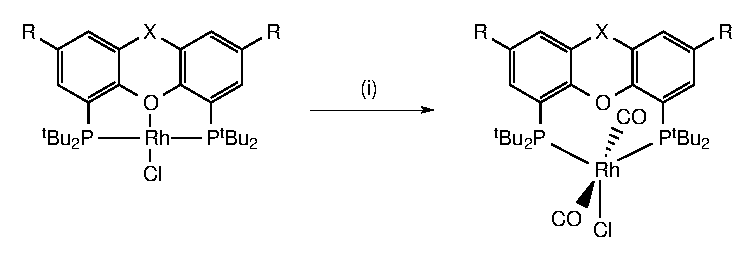
\includegraphics{../Schemes/Rhodiumcarbonyl.eps}
\caption[Reaction of \texorpdfstring{[Rh(\tBuxantphos)Cl{]}} R with carbon monoxide]{Reaction of \texorpdfstring{[Rh(\tBuxantphos)Cl{]}} R with carbon monoxide.}
\vspace{0.2cm}
\label{RhCOpossibilities}
\end{center}
\end{scheme}
\vspace{0.2cm}

Previous reports of the reaction of \Phxantphos{} and DPEphos with \ce{[Rh(CO)2Cl]2} showed the rapid formation of \trans-{[Rh(CO)(diphosphine)Cl]} complexes.\cite{Deb2010}  These complexes appeared in the \phosphorus{} NMR spectrum at 27.3 and 22.6 ppm with \JRhP = 119.2 and 123.5 Hz for \Phxantphos{} and DPEphos respectively.  In the \carbon{} NMR spectrum singlets were observed for the carbonyl at 180.9 and 183.3 ppm for \Phxantphos and DPEphos respectively.  The position of the carbonyl carbon in the \tBuxantphos{} complexes is at 195.5 and 194.9 ppm indicating less shielding which may be a result of the more electron rich rhodium centre in a five-coordinate complex.  The rhodium chemistry of a more sterically demanding version of \Phxantphos{} where the phenyl rings are replaced with \emph{o}-tolyl groups has also been reported.\cite{Williams2011}  Again this complex forms a \trans-[Rh(CO)(diphosphine)Cl] complex.  However the analogous complexes with an iodide replacing the chloride ligand forms a square-pyramidal structure with the oxygen coordinated to the rhodium.  

Dicarbonyl complexes do exist for \Phxantphos{} with [Rh(\Phxantphos)\ce{(CO)2H]} known for \Phsixantphos{} and \Phthixantphos{} as well.\cite{Kranenburg1995}  The diphosphine ligands coordinate in a \emph{bis}-equatorial-\dento{}P,P mode while the hydride occupies an axial site and the two carbonyls in one equatorial and one axial site.  Little difference is observed between the three ligands with the \phosphorus{} peaks between 21.1 and 23.4 (\JRhP = 123.9 - 127.9).  Interestingly although the two carbonyl ligands are inequivalent, only one carbonyl peak was reported despite use of \carbon O occurring as a doublet of triplets at 201.1 with \JRhC{} = 65.7 and \JPC = 10.6 Hz for the \Phxantphos{} complex.  No explanation was given for this but it may be due to the rapid exchange of one of the carbonyl ligands with free CO leading to broadening of the peak.  

\fixme{Still to come: Carbonyl IR results and theoretical analysis of the different structures}

\section{Dioxygen and Oxo Complexes}

The reaction of rhodium(I) complexes with oxygen is well-established with numerous examples published.\cite{Valentine1973, Choy1972}  Many aspects of the oxidation of Wilkinson's complex (\ce{[Rh(PPh3)3Cl]}) to form a distorted octahedral complex with a side-on \hapto{2}-\ce{O2} ligand have been reported including the synthesis\cite{Baird1966, Atlay1980}, degradation\cite{Atlay1983} and use as an oxidation catalyst.\cite{Carlton1983, Read1985}  Numerous other rhodium dioxygen complexes have been reported with monophosphine \cite{Ahijado2005, Aresta1987, Bennett1977, Busetto1977, Gaal1977, Richter2000, Selke1993, Selke1995, Teets2012, Wakatsuki1990} and diphosphine\cite{Banwell2003, James1980,  Mague1977, McGinnety1969, Miller1975, Morvillo1986, Pettinari2002, Slack1979} ligands.  Reports for rhodium dioxygen complexes with heterobidentate\cite{Kashiwabara1997, Lindner1993, Perera1995, Yu2006} and tridentate\cite{Doux2003, Frech2006, Hayashi2013, Lanci2006, Vasapollo1981, Verat2008, Vigalok1996} ligands are also numerous.  However, despite the number of rhodium complexes of \Phxantphos{} and the related ligands no rhodium dioxygen complexes have been reported.  As such we aimed to investigate the reactivity of the [Rh(\POP)Cl] and [Rh(\POP)\ce{(H)2}Cl] (\POP{} = \tBusixantphos{}, \tButhixantphos{} and \tBuxantphos) complexes with oxygen.  

Bubbling air through a \ce{C6D6} solution of each of the [Rh(\tBuxantphos)Cl] complexes resulted in the rapid formation of a new complex as expected (Scheme \ref{Rhodiumdioxygen}).  The same complex formed by reaction of [Rh(\POP)\ce{(H)2}Cl] with air.  With each of the three \tBuxantphos{} ligands the resulting \phosphorus{} NMR spectrum showed a single doublet (39.4 - 40.5) shifted upfield from the [Rh(\tBuxantphos)Cl] complex by between 4.8 and 7.5 ppm (Table \ref{table:dioxygennmr}).  There was a decrease in \JRhP{} of between 37.8 and 41.6 Hz to between 100.7 and 102.2 Hz.  This is consistent with an increase in the oxidation state of the rhodium from +1 to +3 and the corresponding decrease in the s-character of the metal hybrid orbital resulting from the change in coordination geometry from square-planar to octahedral.  

\begin{scheme}[htb]
\begin{center}
\vspace{0.5cm}
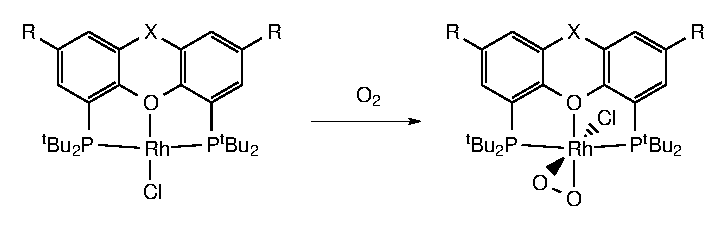
\includegraphics{../Schemes/Rhodiumdioxygen.eps}
\caption[Reaction of \texorpdfstring{[Rh(\tBuxantphos)Cl{]}} R with oxygen]{Reaction of \texorpdfstring{[Rh(\tBuxantphos)Cl{]}} R with oxygen.}
\vspace{0.2cm}
\label{Rhodiumdioxygen}
\end{center}
\end{scheme}
\vspace{0.2cm}

\begin{table}[htbp]
\caption[Selected NMR data for [Rh(\tBuxantphosk)Cl($\eta^2$-\ce{O2}){]}]{Selected NMR data for [Rh(\tBuxantphosk)Cl($\eta^2$-\ce{O2})]}
\vspace{1em}
\label{table:dioxygennmr}
\small
\begin{center}
\begin{tabular}{c c c c c c c c}
\toprule{}
	~~ & \multicolumn{4}{c}{\bfseries{\phosphorus}} & \multicolumn{3}{c}{\bfseries{\carbon{} \emph{O}-ipso}}\\
	\cmidrule(lr){2-5} \cmidrule(lr){6-8}
	\bfseries{Diphosphine}&\bfseries{$\delta/$ppm}&\bfseries{$\Delta\delta/$ppm}&\bfseries{\JRhP}&\bfseries{$\Delta$ \JRhP$/$Hz}&\bfseries{$\delta/$ppm}&\bfseries{$\Delta\delta/$ppm}&\bfseries{\J{} Hz} \\
	\midrule{}
	\tBuSixantphos 		& 39.4 & 4.8 & 102.2 & 37.8 & 166.7 & 2.4 & 9.8\\
	\tBuThixantphos 	& 39.0 & 7.5 & 101.5 & 40.0 & 155.9 & 0.6 & 12.5\\
	\tBuXantphos		& 40.5 & 7.2 & 100.7 & 40.5 & 157.3 & 1.5 & 11.5\\
	\bottomrule{}
\end{tabular}
\end{center} 
\end{table}

The \proton{} and \carbon{} NMR spectra for the three dioxygen complexes showed a loss of symmetry compare to the starting [Rh(\tBuxantphos)Cl] complexes.  While a single peak was observed for the methyl environment for the \tButhixantphos{} complex, two peaks were present for the methyls in the \tBusixantphos{} and \tBuxantphos{} complexes.  Similarly in three cases, two different sets of peaks for the \tBu{} groups were observed.  This is indicative of a loss of the mirror plane that lies along the aromatic system of the ligand, consistent with the proposed structure.  

Interestingly the two methyl groups on the \tBusixantphos{} and \tBuxantphos{} ligands occur in very different positions.  Compared to the [Rh(\tBuxantphosk)Cl] starting material and [Rh(\tBuxantphosk)\ce{(H)2Cl]}, one of the methyls is shifted upfield and the other downfield in both the \proton{} and \carbon{} NMR spectra.  The effect is more pronounced for \tBuxantphos{} than \tBusixantphos{}.  In addition one of the \tBu{} groups in each of the three \tBuxantphos{} ligands is well-resolved as a virtual triplet for all the \proton{} and \carbon{} environments while the other \tBu{} group has a well-resolved virtual triplet for the quaternary carbon while the terminal carbon and protons are broad.

\begin{table}[htbp]
\caption[Comparison of the NMR data for the methyls in \tBusixantphos{} and \tBuxantphos{} rhodium complexes]{Comparison of the NMR data for the methyls in \tBusixantphos{} and \tBuxantphos{} rhodium complexes}
\vspace{1em}
\label{table:dioxygennmr}
\small
\begin{center}
\begin{tabular}{ l c c c c}
\toprule{}
	~~ & \multicolumn{2}{c}{\bfseries{\proton}} & \multicolumn{2}{c}{\bfseries{\carbon}}\\
		\cmidrule(lr){2-3} \cmidrule(lr){4-5}
	\bfseries{Complex}&\bfseries{$\delta/$ppm}&\bfseries{$\delta/$ppm}&\bfseries{$\delta/$ppm}&\bfseries{$\delta/$ppm}\\
		\midrule{}
		{[}Rh(\tBuSixantphosk)Cl]			& 0.07&~ & -0.7~ &~ \\
		{[}Rh(\tBuSixantphosk)Cl(H)\sub{2}]	& 0.17 & 0.10 & -0.7 & -0.9 \\
		{[}Rh(\tBuSixantphosk)\ce{(CO)2}Cl]	& 0.18 & ~&-1.5 & ~\\
		{[}Rh(\tBuSixantphosk)\hapto{2}-\ce{(O2)}Cl] & 0.19 & 0.01 & 0.8 & -4.2 \\
		{[}Rh(\tBuXantphosk)Cl]			& 1.16 & ~ & 33.8 &~\\
		{[}Rh(\tBuXantphosk)\ce{Cl(H)2}]		& 1.25 & 1.22 & 32.4 & 30.4 \\
		{[}Rh(\tBuXantphosk)\ce{(CO)2}Cl]	& 1.24 & ~ & 31.4 &~ \\
		{[}Rh(\tBuXantphosk)\hapto{2}-\ce{(O2)}Cl] & 1.43 & 1.00 & 35.5 & 24.2 \\
	\bottomrule{}
\end{tabular}
\end{center} 
\end{table}

%Unlike the complexes with iPr-xantphos the complexes \ce{[Rh($\eta^3-$tBu-xantphos)Cl]} were unstable in solution over prolonged periods.  Overnight a new resonance appeared in the \phosphorus NMR spectrum, shifted upfield with a much smaller coupling constant (\JRhP{} = 101.5 Hz).  This decrease in coupling constant is consistent with an increase in the oxidation state to rhodium(III).  However, this occurred in dry, degassed \ce{C6D6} which should not be reactive towards the complex.  No signals other than those expected for the ligand were observed in the \proton, \carbon, or \phosphorus{} NMR spectra.  

In the \carbon{} NMR spectra for the [Rh(\tBuxantphos)(\hapto{2}-\ce{O2)Cl]} the shift in the position of the O-\emph{ipso} carbon peak from the free ligand was lower than that reported for the [Rh(\tBuxantphos)Cl] complexes.  In particular the \tButhixantphos{} dioxygen complex exhibited a shift in position of only 0.6 ppm, however the effect is typically reduced for the \tButhixantphos{} ligand system, in fact for [Rh(\tButhixantphos)\ce{(H)2Cl]} a shift of only 0.1 ppm was observed despite a \dento{}\POP{} coordination geometry.  The difference in this may be due to the electron donation from the methyl groups on the aromatic system of \tButhixantphos{} which may mitigate the loss of electron density in the O-\emph{ipso} carbon upon oxygen coordination.  The shifts for \tBusixantphos{} and \tBuxantphos{} are both consistent with \dento{}\POP{} coordination in the dioxygen complexes.  

Dark red crystals were obtained by slow evaporation of a \ce{C6D6} solution of the resulting [Rh(\tBuxantphosk)Cl(\hapto{2}-\ce{O2})] complex (Figure \ref{Crystal:rhodium}).  The crystal structure displayed some substitutional disorder with the dioxygen ligand replaced in approximately 15\% of the sites by an oxo ligand (Figure \ref{Crystal:rhodiumoxo}).  The complexes co-crystallised in the orthorhombic space group \emph{Pbca}.  Crystallographic data is given in Table \ref{crystal:rhodium:data} and selected bond lengths and angles are given in Table \ref{crystal:rhodium:lengths}.


%rhodium(III) complex.  The crystal structure (Figures \ref{Crystal:rhodium}) revealed the presence of a coordinated dioxygen molecule.  The complex crystallised as \ce{[Rh(tBu-xantphos)Cl(}$\eta_2$\ce{-O2})] in the orthorhombic space group \emph{Pbca}.  Selected bond lengths and angles are given in Table \ref{crystal:rhodium:lengths} and crystallographic data is given in Table \ref{crystal:rhodium:data}.  This complex likely formed by slow diffusion of oxygen through the septum sealing the NMR tube.  The crystal structure showed some substitutional disorder with the peroxo ligand substituted for an oxo ligand in approximately 15\% of the sites.  Selected bond lengths and angles for the oxo complex are given in Table \ref{crystal:rhodium:lengths:oxo}.

\begin{figure}[htbp]
\begin{center}
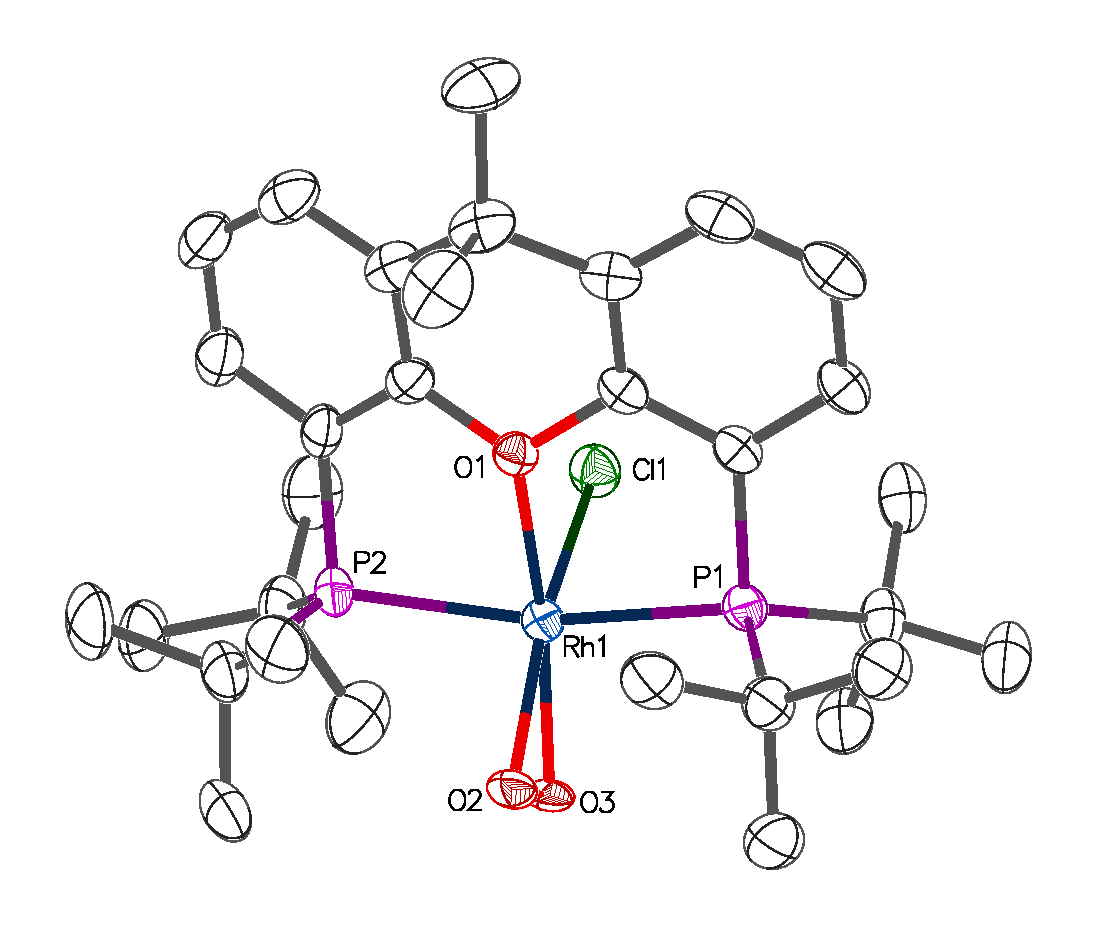
\includegraphics[scale=0.55]{../Crystalstructures/MRMN-Ga-dioxygen.eps}
\caption[X-ray crystal structure of \ce{[Rh(tBu-xantphos)Cl(}$\eta^2$\ce{-O2}){]}]{X-ray crystal structure of \ce{[Rh(tBu-xantphos)Cl(}$\eta^2$\ce{-O2})], hydrogen atoms omitted for clarity.}
\label{Crystal:rhodium}
\end{center}
\end{figure}

\begin{figure}[hbtp]
\begin{center}
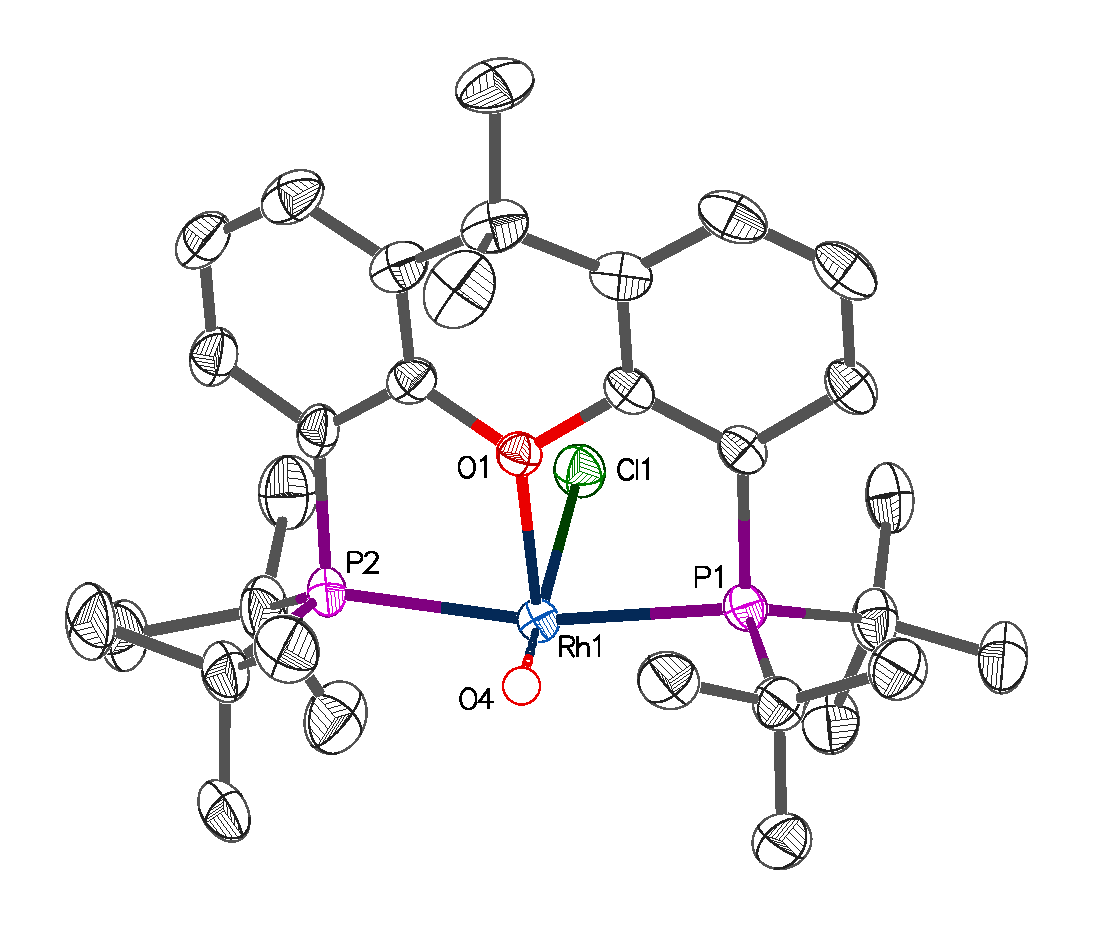
\includegraphics[scale=0.55]{../Crystalstructures/MRMN-Ga-oxo.eps}
\caption[X-ray crystal structure of [Rh(\tBuxantphosk)Cl(O)]{X-ray crystal structure of [Rh(\tBuxantphosk)(O)Cl], hydrogen atoms omitted for clarity.}
\label{Crystal:rhodiumoxo}
\end{center}
\end{figure}

%\begin{figure}[htp]
%\begin{center}
%\vspace{0.5cm}
%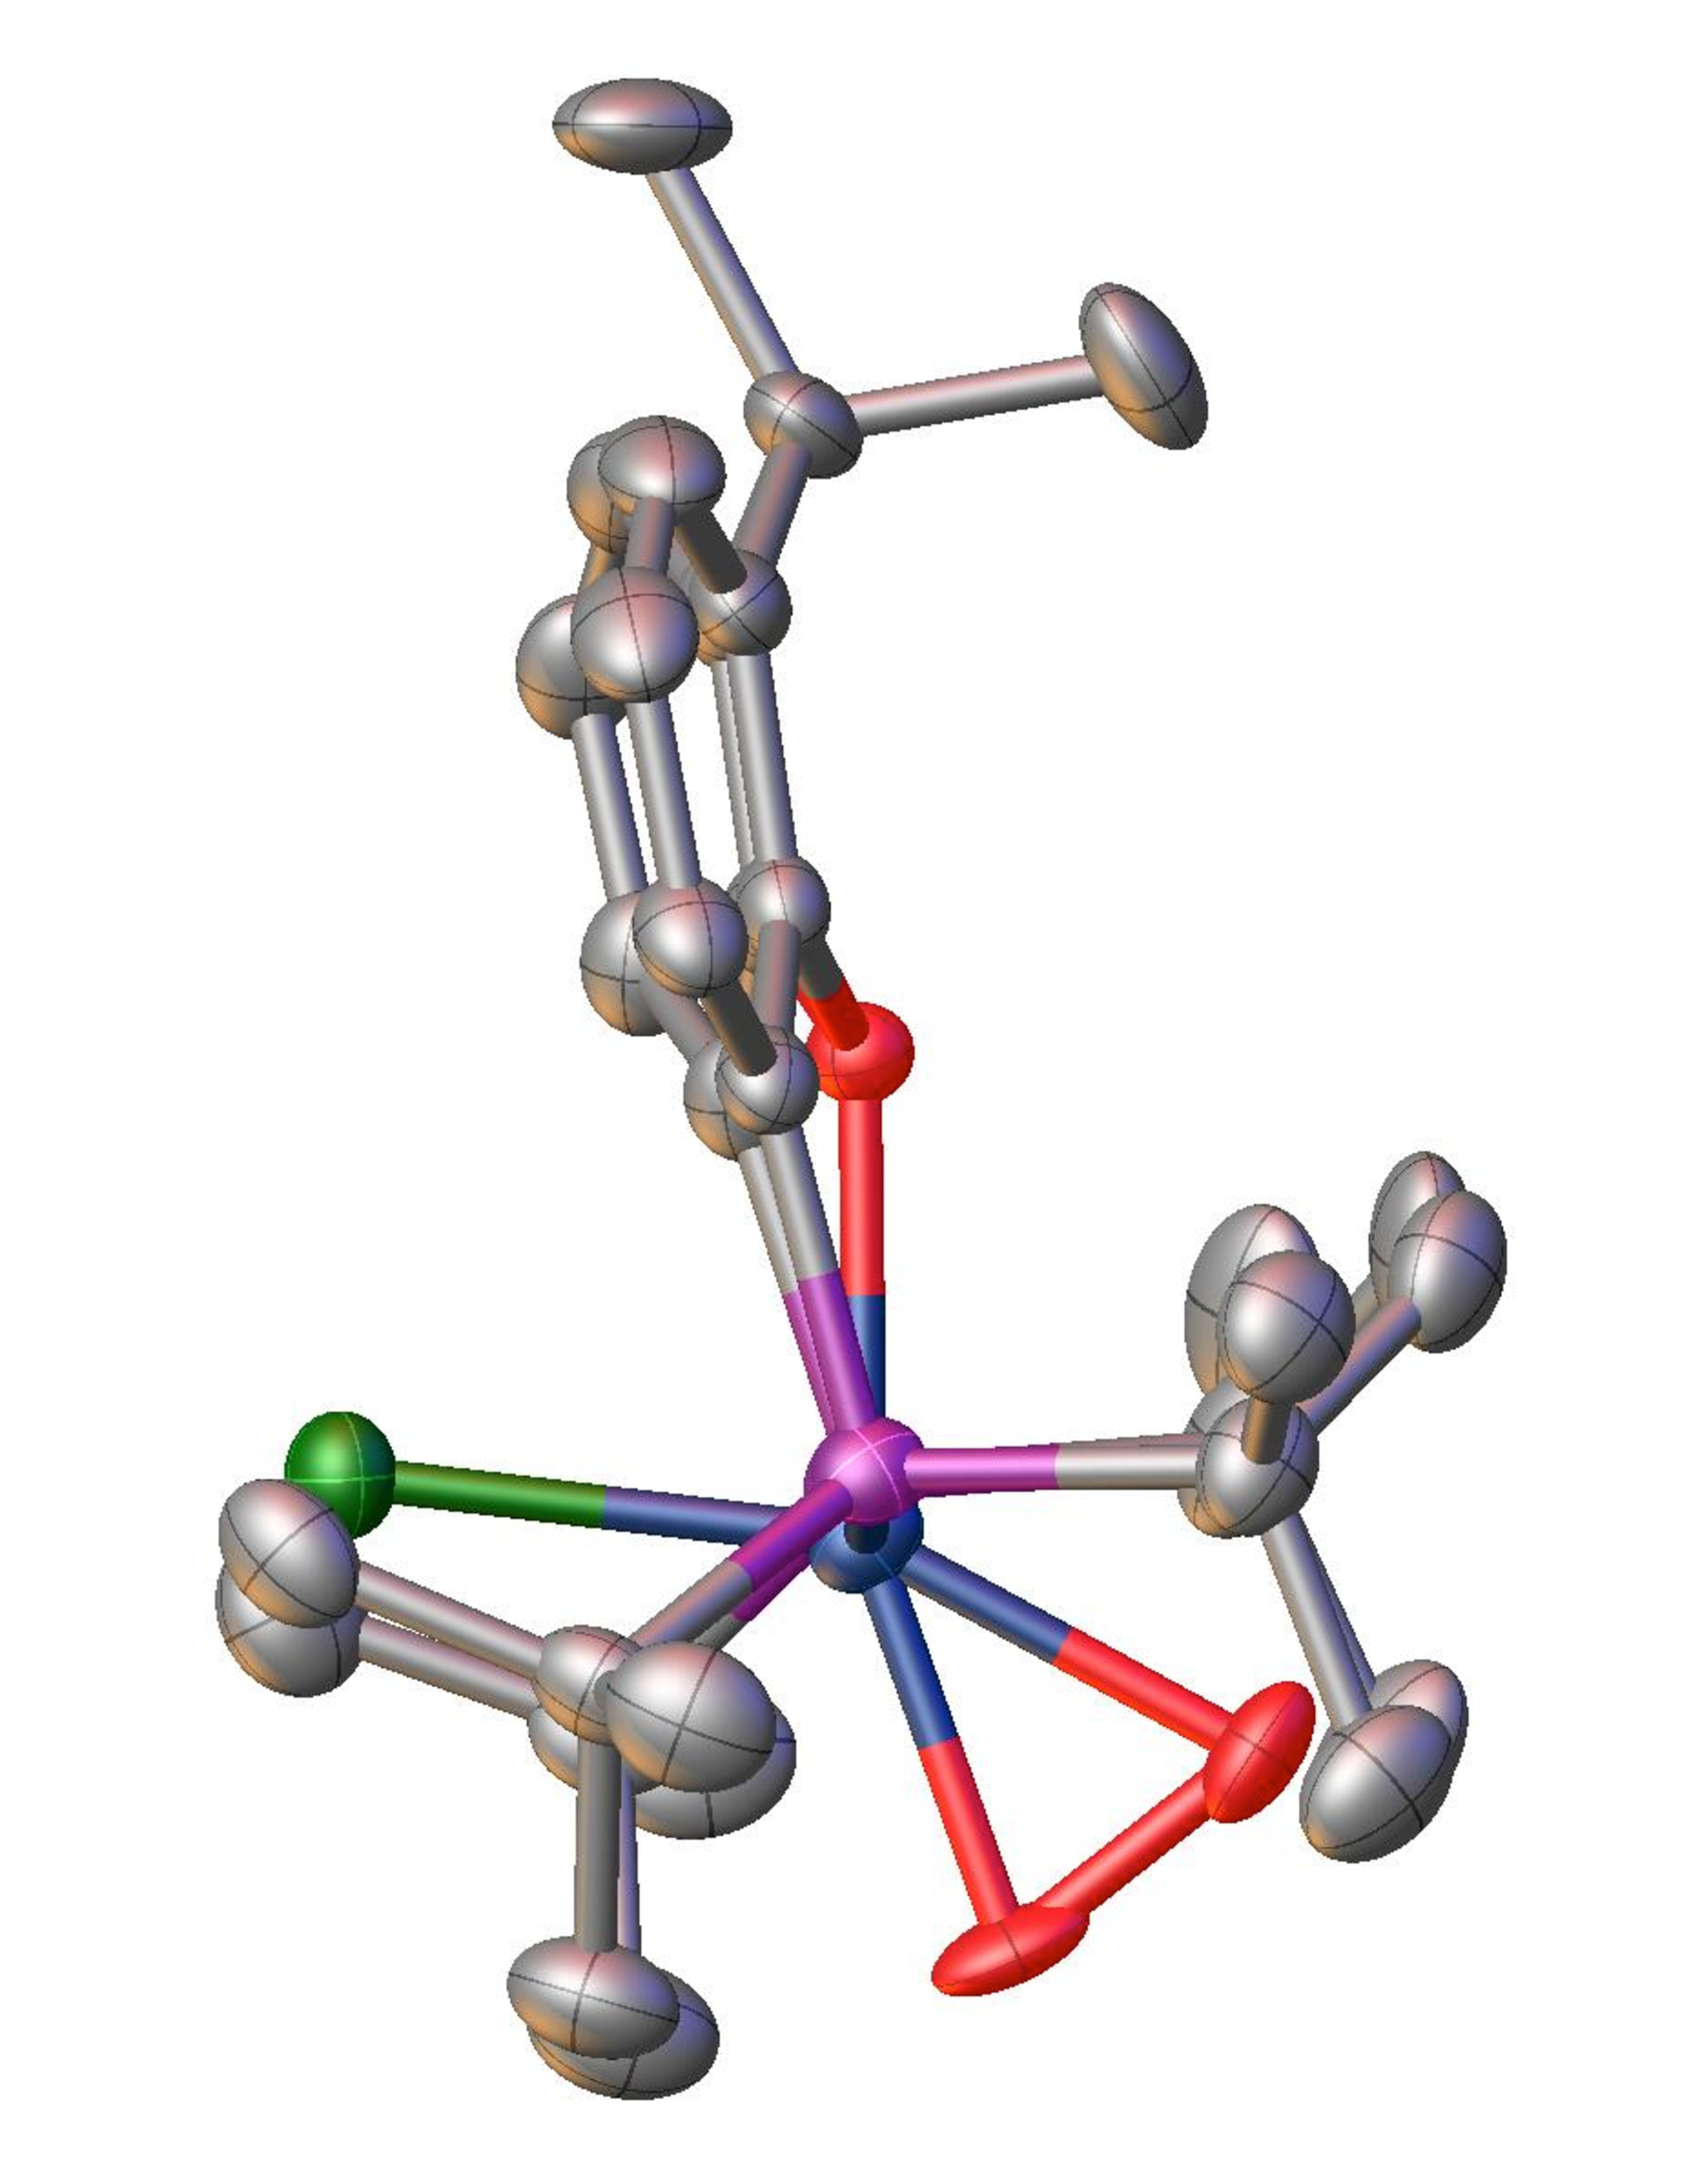
\includegraphics[width=0.4\textwidth]{../Figures/Crystalrhodiumside.pdf}
%\caption[X-ray crystal structure of \ce{[Rh(tBu-xantphos)Cl(}$\eta^2$\ce{-O2}){]} - side view]{X-ray crystal structure of \ce{[Rh(tBu-xantphos)Cl(}$\eta^2$\ce{-O2})], hydrogen atoms omitted for clarity - side view}
%\vspace{0.2cm}
%\label{Crystal:rhodiumside}
%\end{center}
%\end{figure}
%\vspace{0.2cm}

\begin{table}[htbp]
\small
\caption[Crystallographic Data and Structure Refinement of \ce{[Ag(\tButhixantphos)Cl]}]{Crystallographic Data and Structure Refinement of \ce{[Ag(\tButhixantphos)Cl]}} 
\vspace{1em}
\label{crystal:rhodium:data}
\small
\begin{center}
\begin{tabular}{l l}
	\toprule
	\bfseries{Empirical formula}~~& \bfseries{\ce{C31H48ClO2.85P2Rh}}\\
	\midrule
	Formula weight	 							& 666.53\\
	Temperature/K	 							& 120.01(10)\\
	Crystal system	 							& orthorhombic\\
	Space group	 							& Pbca\\
	a$/$\si{\angstrom}							& 11.84223(17)\\
	b$/$\si{\angstrom} 							& 20.2961(3)\\
	c$/$\si{\angstrom}							& 26.8069(4)\\
	$\alpha/$\degrees							& 90\\
	$\beta/$\degrees							& 90\\
	$\gamma/$\degrees							& 90\\
	Volume$/$\si{\angstrom\cubed}  				& 6443.06(17)\\
	Z	 									& 8\\
$\rho$\sub{calc} \si{\milli\gram}$/$\si{\milli\metre\cubed} 	& 1.374\\
\si{\metre}$/$\si{\milli\metre} 						& 6.206\\
F(000)	 									& 2790.0\\
Crystal size$/$\si{\milli\metre\cubed}	 				& 0.1092 x 0.0738 x 0.0159\\
Radiation	 									& CuK$\alpha$ ($\lambda$ = 1.54184)\\
2$\theta$ range for data collection					& 6.594 to 147.8\degrees\\
Index ranges	 								& -14 $\leq$ h $\leq$ 13, -25 $\leq$ k $\leq$ 21, -30 $\leq$ l $\leq$ 33\\
Reflections collected	 							& 45616\\
Independent reflections	 						& 6481 [R\sub{int} = 0.0631, R\sub{sigma} = 0.0332]\\
Data$/$restraints$/$parameters					& 6481$/$399$/$367\\
Goodness-of-fit on F$^{2}$	 					& 1.035\\
Final R indexes [I$>$=2$\sigma$ (I)]	 				& R\sub{1} = 0.0439, wR\sub{2} = 0.1145\\
Final R indexes [all data]	 						& R\sub{1} = 0.0550, wR\sub{2} = 0.1226\\
Largest diff. peak/hole / e \si{\per\angstrom\cubed}		& 1.40/-0.78	\\
	\bottomrule
\end{tabular}
\end{center}
\end{table}

\begin{table}[htp]
\caption[Selected bond distances (\AA) and angles (\degrees) of \ce{[Rh(tBu-xantphos)Cl(}$\eta^2$\ce{-O2}){]}]{Selected bond distances (\AA) and angles (\degrees) of \ce{[Rh(tBu-xantphos)Cl(}$\eta^2$\ce{-O2})]}
\vspace{1em}
\label{crystal:rhodium:lengths}
\small
\begin{center}
\begin{tabular}{l l l l}
	\toprule
	\multicolumn{2}{l}{\bfseries{~Bond distances (\si{\angstrom})}} & \multicolumn{2}{c}{\bfseries{Bond angles (\degrees)}} \\
	\midrule		
	P1-Rh & 2.3391(8)	& P1-Rh-P2 & 166.01(3) \\
	P2-Rh & 2.3237(9)	& Cl1-Rh-O2 & 158.18(10)\\
	O1-Rh & 2.193(2)	& Cl1-Rh-O4 & 161.2(3)\\
	O2-Rh & 2.016(3)	& O1-Rh-O3 & 161.33(12)\\
	O3-Rh & 1.962(3)	& Ring1-Ring2 & 26.65(12)\\
	Cl1-Rh & 2.3871(9)	& & \\
	O2-O3 & 1.424(5)	& & \\
	\bottomrule{}
\end{tabular}
\end{center}
\end{table}


The oxygen-oxygen bond lengthens upon coordination due to back-bonding from the metal into the anti bonding $\pi*$-orbital.  In the crystal structure the O2-O3 bond length is 1.424(5) \si{\angstrom} lengthened by 0.21 \si{\angstrom} from the bond length in molecular oxygen of 1.21 \si{\angstrom}.  This length is typical for rhodium dioxygen complexes with the average O-O bond length of 1.423 \A.  
The Rh-O bond lengths for the dioxygen ligand are different with the oxygen \trans{} to chloride having longer bond length by 0.054 \A.  The oxygen \trans{} to chloride has a typical Rh-O bond length for rhodium dioxygen complexes (average = 2.017 \A), while the oxygen \trans{} to the ether bridge is shorter than average with a length of 1.962(3) \A.  This shorter bond is likely the result of the low \trans{} influence of the ether oxygen.  Only threes complexes with shorter Rh-O bonds for a dioxygen complex have been reported (Figure \ref{ShorterRhOcomplexes}).\cite{Lindner1993b, Penner2011, Wechsler2012} These complexes have the dioxygen atoms \trans{} to nitrogen or oxygen donor atoms, which are known to have a very low \trans{} influence.  Of the 1384 crystals structures with Rh-O bonds currently in the CCDC only 19 have Rh-O bonds shorter than the Rh-O bond \trans{} to the ether bridge in this structure.  All of the crystals structures with shorter Rh-O bond lengths for any oxygen environment have the oxygen \trans{} to weak ligands with nitrogen or oxygen donor atoms.

\begin{figure}[htp]
\begin{center}
\vspace{0.5cm}
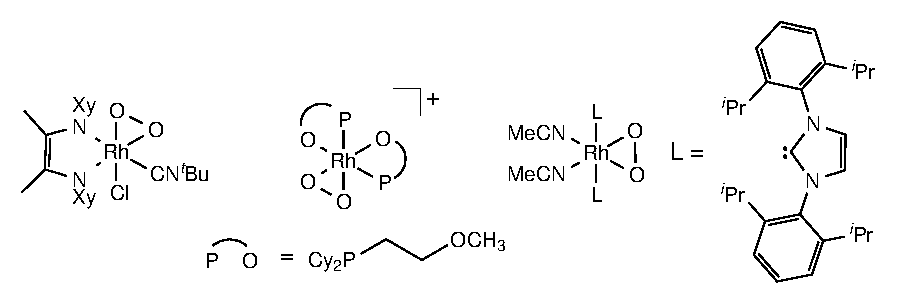
\includegraphics{../Figures/OtherRhO2complexes.eps}
\caption[Rhodium complexes with shorter Rh-O bonds than \texorpdfstring{[Rh(\tBuxantphos)(\hapto{2}-\ce{O2})Cl{]}} R]{Rhodium complexes with shorter Rh-O bonds than \texorpdfstring{[Rh(\tBuxantphos)(\hapto{2}-\ce{O2})Cl{]}} R}
\vspace{0.2cm}
\label{ShorterRhOcomplexes}
\end{center}
\end{figure}
\vspace{0.2cm}

The complex shows two distinct methyl environments in the \proton{} and \carbon{} NMR spectra indicating a loss of symmetry with two distinct faces of the \tBuxantphos{} ligands (Table \ref{table:dioxygennmr}.  From the crystal structure we can clearly see that the chloride ligand sits on the same side as the concave face of the ligand while the peroxo ligand occupies the position pseudo-\emph{trans} to the oxygen bridge of the ligand.  This geometry leaves more space \emph{trans} to the chloride resulting in the curvature of the ligand to occupy this free space and the tipping of the methyl groups away from the chloride.  The angle O1-C(bridge)-\emph{C}\ce{H3} is very different for the two methyl groups; 165.9(3) and 94.7(3) for the concave and convex methyls respectively and dihedral angles to the first C-H in the aromatic ring of -24.8 and -42.8\degrees.  This positioning results in quite different chemical environments for the two methyl groups resulting in the two different NMR environments.  

%Discussion of xantphos dioxygen complexes.
Although rhodium xantphos{} complexes are well-studied due to their high catalytic activity and selectivity for hydroformylation, to the best of our knowledge, no rhodium dioxygen complexes have been reported with xantphos or any xantphos derived ligands.  Indeed only one transition metal complex with a xantphos related ligand and an \hapto{2} dioxygen ligand has been reported; [Ru(\Phxantphos)\ce{(PPh3)(\hapto{2}-O2)H]BAr4^F}.\cite{Ledger2010}  These complexes were formed by reaction of the [Ru(\Phxantphos)\ce{PPh3HCl]} with \ce{NaBAr4^F} followed by filtration then stirring in the air for 10 mins.  Similarly to the rhodium \tBuxantphos{} complexes the \emph{mer}-\dento{}\emph{P,O,P} coordination is retained upon reaction with oxygen.  The dioxygen ligand occupies the site \trans{} to the hydride where the chloride had previously been located.  

As previously mentioned the X-ray crystal structure of [Rh(\tBuxantphos)(\hapto{2}-\ce{O2})Cl] contained substitutional disorder with approx. 15\%{} of the dioxygen molecules replaced by an oxo group (Figure \ref{Crystal:rhodiumoxo}).  The oxo complex shows a slightly distorted square-based pyramid structure with the ether bridge of the \tBuxantphos ligand occupying the apex and \trans{} coordination of the phosphorus atoms.  The rhodium oxo bond (1.669(10) \A) is much shorter than the rhodium peroxo bond lengths consistent with a higher bond order.  In addition the rhodium oxo bond is the shortest crystallographically determined Rh-O bond.  

To the best of our knowledge this is the first example of crystallographic evidence for a rhodium(III) oxo complex.  Only one crystal structure for a rhodium oxo complex has been reported, which is a rhodium(V) system (Figure \ref{Kaczul}).\cite{Gangopadhyay2010}  The literature structure shows a rhodium(V) dimer supported by two oxo ligands, a DMSO ligand and a oxygen-nitrogen heterobidentate ligand.  The oxo \trans{} to the DMSO ligand has a bond length of 1.701(5) \A, while the oxo \trans{} to the nitrogen donor is slightly longer at 1.712(5) \A.  Both of these are very slightly longer than the Rh-O bond length in the [Rh(\tBuxantphos)(O)Cl] structure (1.669(10) \A).  The average bond length for a transition metal oxo is 1.689 \A{} with a lower quartile at 1.671 \A.  This indicates that the bond length for the rhodium oxo is in the lowest quarter on crystallographically determined bond lengths for transition metal oxo complexes however, the bond is well within the range (1.106 - 2.956 \A).  

\begin{figure}[htb]
\begin{center}
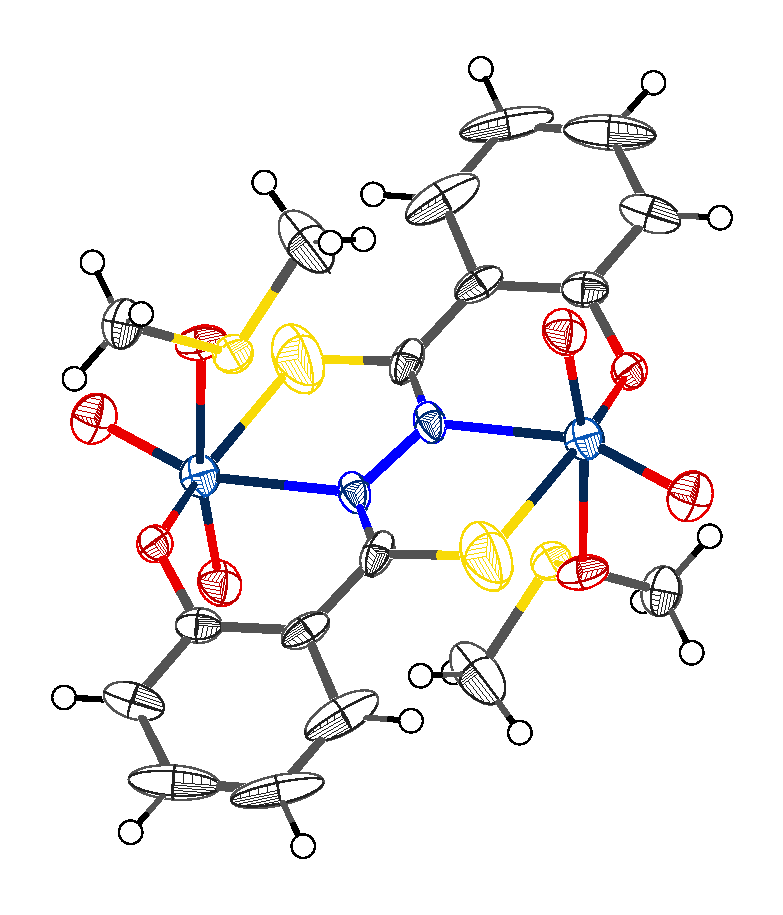
\includegraphics[scale=0.7]{../Othercrystals/KACZUL.eps}
\caption[Previously reported rhodium oxo crystal structure]{Previously reported rhodium oxo crystal structure.\cite{Gangopadhyay2010} Hydrogen atoms omitted for clarity}
\vspace{0.2cm}
\label{Kaczul}
\end{center}
\end{figure}
\vspace{0.2cm}

Transition-metal oxo complexes have long been studied as they have been implicated to have roles in  biological systems,\cite{Lipscomb1994, Merkx2001, Tinberg2011, Montellano2010} C-H activation\cite{Balcells2010, Borovik2011} and various oxidation reactions\cite{Holm1987, Atlay1983, Poverenov2008}.  A terminal oxo ligand is a very strong $\pi$-donor ligand, thus the strongest coordination occurs with high oxidation state, early transition metals\cite{Anderson2004}.  Indeed a review of transition-metal oxo complexes published in 1987 stated that ``M=O groups are stabilised at metal centres with an oxidation state of no less than +4 and no more than four d electrons''.\cite{Holm1987}  This has led to the proposition of an "oxo-wall" a barrier between groups 8 and 9 preventing the formation of tetragonal oxo complexes for group 9-11 transition metals.\cite{Winkler2011}  This effect arises as the orbital splitting in a octahedral oxo complex lowers the symmetry of the t\sub{2g} orbitals to b\sub{2}(d\sub{xy}) and e(d\sub{xz},d\sub{yz}) and the metal-ligand anti bonding e\sub{g} orbitals to b\sub{1}(d\sub{x\superscript{2}-y\superscript{2}}) and a\sub{1}(d\sub{z\superscript{2}}).  with the e(d\sub{xx}, d\sub{yz}) and d\sub{z\superscript{2}} orbitals destabilised.\cite{Betley2008}  The more d-electrons present, the lower the bond order to the oxo resulting in decreased stability.  The [Rh(\tBuxantphos)(O)Cl] complex is of trigonal bipyramidal geometry so does not violate the oxo-wall proposition.  Indeed the poor electron donation from the central ether bridge may lead to increased stability compared to other square-pyramidal structures.  

Despite the instability of terminal oxo complexes for the late-transition metals some examples do exist.  A platinum(II) complex with a P,C,N pincer ligand was reacted with a freshly prepared acetone solution of dioxirane resulting in formation of a platinum (IV) oxo complex (Figure \ref{Rhodiumotheroxo}).\cite{Poverenov2008}  This complex degrades over a period of 7-10 hours \emph{via} an intramolecular oxygen transfer reaction from the platinum to the phosphorus atom.  The oxo also readily reacts with water (forming a bishydroxy, aquo complex), hydrogen (liberating water), carbon monoxide (forming \ce{CO2} and a carbonyl complex), potassium hydride (to form a hydroxy complex) and oxidises triphenyl phosphine.  Thus exhibiting a range of different potential uses for late transition metal oxo complexes.  A very well known iridium(V) oxo complex has also been reported, in this case the oxo complex was synthesised by reaction of \ce{[Ir(mes)3]} (mes = mesityl) with trimethylamine oxide (Figure \ref{Rhodiumotheroxo}).\cite{Motherwell1993}  A rhodium(III) oxo-complex was recently reported by Caulton \emph{et} al. from reaction of rhodium(III) hydride complex with a metalled PNP ligand reacting with trimethylamine oxide, pyridine \emph{N}-oxide or \ce{N2O}.\cite{Verat2008, Tsvetkov2013}  This complex undergoes oxo transfer reactions with trimethylphosphine and carbon monoxide.

\begin{figure}[htb]
\begin{center}
\vspace{0.5cm}
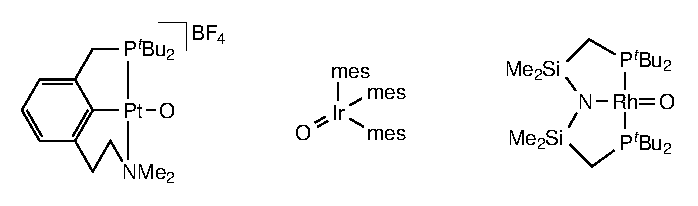
\includegraphics{../Figures/Rhodiumotheroxo.eps}
\caption[Previously reported late-transition metal oxo complexes]{Previously reported late-transition metal oxo complexes. mes = 2,4,6-trimethylphenyl.}
\vspace{0.2cm}
\label{Rhodiumotheroxo}
\end{center}
\end{figure}
\vspace{0.2cm}

Attempts to synthesise the [Rh(\tBuxantphos)(O)Cl] series of complexes by oxidation of the [Rh(\tBuxantphos)Cl] were made following the discovery of the oxo in the crystal structure of [Rh(\tBuxantphos)(\hapto(2)-\ce{O2})Cl].  Oxidation was attempted using trimethylamine oxide as this has been used previously in the synthesis of late-transition metal oxo complexes\cite{Motherwell1993, Tsvetkov2013} and the by-product of trimethylamine should be a poor ligand and result in little reactivity.    Reaction between [Rh(\tBusixantphos)Cl] and trimethylamine oxide resulted in the immediate formation of the [Rh(\tBusixantphos)(\hapto(2)-\ce{O2})Cl] complex, together with a small amount of the ligand oxide, over time peaks due to the [Rh(\tBusixantphos)Cl] complex began to reappear.  This result may be due to the incomplete dissolution of [Rh(\tBusixantphos)Cl] in the \ce{CD2Cl2} reaction solvent meaning that amount in solution was over-oxidised before the remainder dissolved.  Unfortunately as [Rh(\tBusixantphos)Cl] is a dark brown colour it is challenging to gauge full dissolution.  

Reaction between [Rh(\tButhixantphos)Cl] and trimethylamine oxide resulted in a mixture of compounds.  Analysis by \phosphorus{} NMR showed 22.9\%{} free \tButhixantphos{} ligand indicating possible degradation of the rhodium complexes formed, 8.6\%{} was [Rh(\tBusixantphos)(\hapto(2)-\ce{O2})Cl], 64.4\% starting material and a new complex at 40.9 ppm (\JRhP{} = 90.4 Hz) made up 4.1\% of the reaction mixture.  After 10 days no [Rh(\tButhixantphos)Cl] or the unidentified complex remained and the reaction mixture was primarily the dioxygen complex and a further new complex at 74.1 ppm (\JRhP{} = 116.3 Hz).  

The reaction of [Rh(\tBuxantphos)Cl] with trimethylamine oxide was initially carried out at -80 \degC{} in order to prevent over-oxidation.  However, initially the slow generation of the dioxygen species was observed with no evidence for any intermediate or otherwise.  The reaction was allowed to warm to room temperature and after 24 hours a small amount of a complex at 42.6 ppm (\JRhP{} = 90.4 Hz).  However, around 50\%{} of the reaction mixture was the dioxygen complex and the remainder was the Rh(I) starting material.  Addition of further trimethylamineoxide resulted in the slow (1 week) conversion of the Rh(I) chloride into the unknown complex.  Similarly to the \tButhixantphos{} reaction this reaction slowly converts into a species at 75.1 ppm (\JRhP{} = 116.3 Hz).  

The NMR spectra of the first unknown complex for the oxidation of [Rh(\tBuxantphos)Cl] and [Rh(\tButhixantphos)Cl] are very similar.  In the \phosphorus{} NMR a doublet was observed slightly downfield of the peroxy complex.  The values of \JRhP{} were identical with either ligand (90.4 Hz).  The decrease from the values in the rhodium(I) complex (142.3 and 140.0 Hz for \tBuxantphos{} and \tButhixantphos{} respectively) clearly indicates oxidation to a rhodium(III) species.  \fixme{talk about \proton{} and \carbon{} if possible}  Mass spectrometry was performed on all three reaction mixtures.  In all cases a molecular ion peak was observed consistent in both mass charge ratio and isotopic pattern, with indicative of an oxo complex ionising \emph{via} loss of a chloride ligand was observed.

Phosphine ligands can act as pi-acceptor ligands with back-donation into P-C $\sigma*$-bonds which have $\pi$ symmetry.  While the bonding of \tBu{} phosphines is generally dominated by the $\sigma$-donation the \tBuxantphos{} ligands also have an aromatic substituent which is enhance the back-bonding relative to trialkylphosphines.  Terminal oxo ligands are strong $\pi$-donor ligands\cite{Betley2008} so we would expect that coordination of an oxo ligand would increase the electron density on the metal thereby increasing the back-donation to the phosphorus atoms.  This would result in a longer P-M bond and thus lower coupling Rh-P coupling constants are observed in the oxo complexes than in the dioxygen or dihydrogen complexes.  Hence, based on the data discussed we tentatively postulate the identity of the first unknown complex as a square pyramidal rhodium(III) oxo complex (Scheme \ref{Rhodiumoxo}).

\begin{scheme}[htb]
\begin{center}
\vspace{0.5cm}
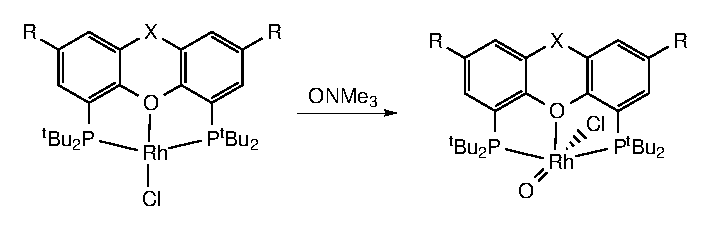
\includegraphics{../Schemes/Rhodiumoxo.eps}
\caption[Reaction of \texorpdfstring{[Rh(\tBuxantphos)Cl{]}} R with trimethylamine oxide]{Reaction of \texorpdfstring{[Rh(\tBuxantphos)Cl{]}} R with trimethylamine oxide}
\vspace{0.2cm}
\label{Rhodiumoxo}
\end{center}
\end{scheme}
\vspace{0.2cm}

Late-transition metal oxo complexes are generally considered unstable and likely to undergo further reaction.  The reactions of [Rh(\tBuxantphos)Cl] with trimethylamine oxide were performed in \ce{CD2Cl2} as previously discussed (see Section \fixme{refer to ligand protonation section}) halocarbon molecules are not stable for extended periods of time in the light, undergoing a photo-catalysed degradation forming small amounts of hydrochloric acid (deuterium chloride in the case of NMR solvents).\cite{Yano1977}  Hereby we propose that the oxo complex likely reacted with the small amounts of deuterium chloride that formed over time, thus producing a hydroxy ligand (Scheme \ref{Rhodiumhydroxy}).  The remaining coordination site on the metal would then likely be occupied by the chloride ion.  The platinum oxo complex reported by Milstein \emph{et} al. underwent reaction with water to form a \emph{bis}-hydroxy complex while the rhodium oxo reported by Caulton \emph{et} al. underwent metallation of one of the \tBu{} substituents on the phosphorus donor also forming a hydroxy ligand.\cite{Verat2008}  

\begin{scheme}[htb]
\begin{center}
\vspace{0.5cm}
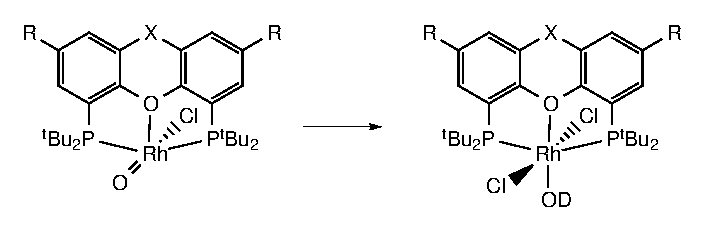
\includegraphics{../Schemes/Rhodiumhydroxy.eps}
\caption[Reaction of \texorpdfstring{[Rh(\tBuxantphos)(O)Cl{]}} R with hydrochloric acid]{Reaction of \texorpdfstring{[Rh(\tBuxantphos)(O)Cl{]}} R with hydrochloric acid}
\vspace{0.2cm}
\label{Rhodiumhydroxy}
\end{center}
\end{scheme}
\vspace{0.2cm}

Unfortunately due to the time constraints of a PhD the formation of the rhodium oxo complexes was unable to be studied in more depth.  

\section{Conclusion}

%\section{Iridium Complexes}
%\label{section:experimental:iridium}

%Reaction between \ce{[Ir(COE)2Cl]2} and iPr-xantphos resulted in an iridium(III) complex with the iPr-xantphos coordinating tetradentate through the phosphines, oxygen and a metalled methyl of an isopropyl group.\cite{Esteruelas2013}  Also coordinated are the original chloride ligand and a hydride formed in the metallation.  The reaction likely proceeds via a \ce{[Ir($\eta^3-$iPr-xantphos)Cl]} and then metallation occurs.  However, no spectroscopic evidence for the \ce{Ir($\eta^3-$iPr-xantphos)Cl]} was reported.  Given that metallation occurs on platinum for the reaction between the dioxygen complex and carbon monoxide \fixme{reference} it was expected that metallation should occur in a relatively facile manner when the tBu-xantphos ligands were reacted with \ce{[Ir(COE)2Cl]2}.  

%However, when the reactions were carried out they proved to be very slow, and gave intractable mixtures of products.  In each case a large number of hydride resonances were observed indicating that metallation had occurred however, the nature of the complexes was unable to be determined.  The reactions became dark relatively rapidly though they continued to react after this colour change was observed.  The \ce{[Rh($\eta^3-$tBu-xantphos)Cl]} complex was dark red so the colour change is not necessarily a sign of degradation of the iridium starting material.  














